%% LaTeX2e class for student theses
%% thesis.tex
%%
%% Karlsruhe University of Applied Sciences
%% Faculty of  Computer Science and Business Information Systems
%% Distributed Systems (vsys)
%%
%% Prof. Dr. Christian Zirpins
%% christian.zirpins@hs-karlsruhe.de
%%
%%
%% Version 0.2, 2017-11-15
%%
%% --------------------------------------------------------
%% | Derived from sdqthesis by Erik Burger burger@kit.edu |
%% --------------------------------------------------------

%% Available languages: english,ngerman
%% Available modes: draft,final (see README)
\documentclass[ngerman,final]{vsysthesis}

% Use space between paragraphs
%\KOMAoption{parskip}{half+}

%% ---------------------------------
%% | Information about the thesis  |
%% ---------------------------------

%% Name of the author
\author{Fabian Sorn}

%% Title (and possibly subtitle) of the thesis
\title{
	Benchmarking, analysis, and optimization of Python-based graph
	library performance
}

%% Type of the thesis
\thesistype{Bachelor Thesis}

%% Change the institute or subject area here, ``VSYS'' is default
% \myinstitute{Institute for \dots}

%% You can put a logo in the ``logos'' directory and include it here
% \grouplogo{myfile}

%% The reviewers are the professors that grade your thesis , ``Zirpins'' is default
%\reviewerone{Prof. A}
%% reviewer two (can be omitted)
\reviewertwo{Prof. B}

%% The advisor is usually extern (can be omitted)
\advisorone{}
% The second advisor (can be omitted)
\advisortwo{Dipl.-Inform. D}

%% Please enter the start end end time of your thesis
\editingtime{10. November 2019}{10. March 2020}

\settitle

%% --------------------------------
%% | Settings for word separation |
%% --------------------------------

%% Describe separation hints here.
%% For more details, see
%% http://en.wikibooks.org/wiki/LaTeX/Text_Formatting#Hyphenation
\hyphenation{
% me-ta-mo-del
}

%% --------------------------------
%% | Bibliography                 |
%% --------------------------------

%% Use biber instead of BibTeX, see README
\usepackage[citestyle=numeric,style=numeric,backend=biber]{biblatex}
\addbibresource{thesis.bib}

%% --------------------------------
%% | Listings                     |
%% --------------------------------
 
\usepackage{listings}
\usepackage[utf8]{inputenc}
\usepackage{xcolor}

\definecolor{commentcolor}{HTML}{2e7d32}
\definecolor{numbercolor}{HTML}{607d8b}
\definecolor{stringcolor}{HTML}{e65100}
\definecolor{keywordcolor}{HTML}{4527a0}
\definecolor{backcolor}{HTML}{f7f9fa}
 
\lstdefinestyle{mystyle}{
    backgroundcolor=\color{backcolor},
    commentstyle=\color{commentcolor},
    keywordstyle=\color{keywordcolor},
    numberstyle=\tiny\color{numbercolor},
    stringstyle=\color{stringcolor},
    basicstyle=\fontsize{11}{13}\selectfont\ttfamily,
    breakatwhitespace=false,
    breaklines=true,
    captionpos=b,
    keepspaces=true,
    numbers=left,
    numbersep=5pt,
    showspaces=false,
    showstringspaces=false,
    showtabs=false,
    tabsize=2
}
 
\lstset{style=mystyle}

\newcommand{\inlinecode}[2]{
  \colorbox{backcolor}{
    \lstinline[language=#1]$#2$
  }
}

%% --------------------------------
%% | Glossaries                   |
%% --------------------------------

%% Use glossaries (optional)
\makeglossaries
%% Load glossary definitions from file
\loadglsentries{glossentries.tex}

%% ====================================
%% ====================================
%% ||                                ||
%% || Beginning of the main document ||
%% ||                                ||
%% ====================================
%% ====================================
\begin{document}

%% Set PDF metadata
\setpdf

%% Set the title
\maketitle

%% The Preamble begins here
\frontmatter

%% LaTeX2e class for student theses: Declaration of independent work
%% sections/declaration.tex
%%
%% Karlsruhe University of Applied Sciences
%% Faculty of  Computer Science and Business Information Systems
%% Distributed Systems (vsys)
%%
%% Prof. Dr. Christian Zirpins
%% christian.zirpins@hs-karlsruhe.de
%%
%%
%% Version 0.2, 2017-11-15
%%
%% --------------------------------------------------------
%% | Derived from sdqthesis by Erik Burger burger@kit.edu |
%% --------------------------------------------------------


\thispagestyle{empty}
\null\vfill
\noindent\hbox to \textwidth{\hrulefill}
\iflanguage{english}{I declare that I have developed and written the enclosed
thesis completely by myself, and have not used sources or means without
declaration in the text.}%
{Ich versichere wahrheitsgemäß, die Arbeit
selbstständig angefertigt, alle benutzten Hilfsmittel vollständig und genau
angegeben und alles kenntlich gemacht zu haben, was aus Arbeiten anderer
unverändert oder mit Änderungen entnommen wurde.}


%% ---------------------------------------------
%% | Replace PLACE and DATE with actual values |
%% ---------------------------------------------
\textbf{PLACE, DATE}
\todo{Please replace with actual values}
\vspace{1.5cm}

\dotfill\hspace*{8.0cm}\\
\hspace*{2cm}(\theauthor)
\cleardoublepage


\setcounter{page}{1}
\pagenumbering{roman}

%% ----------------
%% |   Abstract   |
%% ----------------

%% For theses written in English, an abstract both in English
%% and German is mandatory.
%%
%% For theses written in German, a German abstract is sufficient.
%%
%% The text is included from the following files:
%% - sections/abstract

\includeabstract

%% ------------------------
%% |   Table of Contents  |
%% ------------------------
\tableofcontents

\listoffigures
\listoftables

%% ------------------------
%% | Glossary/Acronyms    |
%% ------------------------

% print glossary (optional)
\printglossary[title=Glossar]

% print acronyms (optional)
\printglossary[type=\acronymtype]

%% -----------------
%% |   Main part   |
%% -----------------

\mainmatter

%% ==============================================
%%               Introduction
%% ==============================================
%% Author: Fabian Sorn
%% ==============================================

\chapter{Introduction}
\label{ch:Introduction}

The following chapter will provide an introduction into this work. First the setting in which the work is done, will be described, starting with the orgranisation followed by the team. Afterwards the fundamental problem and the goal of this work will be explained, rounded up by an overview about the structure of the following chapters.




%% ==============================================
%%               Motivation
%% ==============================================

\section{Motivation}
\label{sec:Introduction:Motivation}

The big advantage that the raise of computing brought with it, was, that complex mathematical tasks, could be performed in very little time. Since the beginnings, a lot has happened and computers got much more powerful. Even with these improvements, the question of good performance could not be more relevant as today. We have to make sure, that the hardware and our algorithms are fast enough, to keep up with the tasks we we want to accomplish. This demand is especially relevant in the scientific world, where often gigantic data sets have to be filtered, recorded and analyzed. A popular tool for such work are software products, that allow us to visualize data as graphs, since visualization allows us to have a much deeper insight into the data we want to understand. As with any type of software, the performance of graphs has to keep up with our high demands. One of the places, where this couldn't become more clear, is CERN, where the fundamental question the following work is based on, was researched.




%% ==============================================
%%                    CERN
%% ==============================================

\section{CERN}
\label{sec:Introduction:CERN}

The \gls{cern} is one of the biggest and most well known research facilities in the world. It is most known as the host of one of the world most complex and astonishing machines, the \gls{lhc} as well as the birth place of the \gls{web}, on which we rely on daily everywhere around the world. \cite{Cern}
These and many more achievements and projects all contribute to the central mission at \gls{cern}: Finding out, what our universe is made of. To find answers to this question, \gls{cern} brings together over 17500 people from all over the world, to work together in many different fields including physics, engineering, computer science and more. Today, \gls{cern} counts 23 member states that collaborate on decisions made at in the organisation every day \cite{CernWhoWeAre}.

\gls{cern}'s roots can be traced back to the 1940's, when a hand full of scientists saw the needs for Europe to advance its role in the scientific world by hosting its own research facility for physics. Starting with 12 original member states, \gls{cern} originally was founded based on this vision in 1954 located at the franco-swiss border, as the \emph{Conseil Européen pour la Recherche Nucléaire}, leading to today's well recognized acronym \gls{cern}. Until today, these member states are contributing to \gls{cern}'s financing, organisation and foundations to achieve its goals to expand the boundaries of human knowledge. \cite{CernOurHistory}




%% ==============================================
%%                 BE-CO-APS
%% ==============================================

\section{Beams Controls Applications}
\label{sec:Introduction:BE-CO-APS}

\gls{cern}'s main focus for research is particle physics. To continuously improve our knowledge in this field, \gls{cern} is operating the world's most powerful particle accelerator called \gls{lhc}. The \gls{lhc} allows us to gain a much deeper insight into the subatomic structure of the world around us bringing us closer to understanding the inner workings of our universe. \gls{cern} itself is devided into different departments which have their own purposes. The \gls{be} is responsible for developing software and hardware instruments for the accelerator complex. \cite{CernBeamsDep}

The \gls{lhc}'s task is to produce and accelerate two beams of charged particles, travelling in opposite directions. To achieve this,it is constructed as two circular pipes containing a vacuum, which are surrounded by magnets. The magnetic field created by these magnets can accelerate and steer particles passing by. If a beam of particles is injected into the accelerator, the strength of the magnetic field is increased with every round the beam travels in the accelerator, until the beam reaches speeds very close to the speed of light. Is this level of energy reached, the next step is to make particles from the two beams collide with each other. \gls{cern} is operating four experiments, Atlas, CMS, Alice and LHCb, where the particles can be led to collission. The particles detectors then can record the results of the collisions in great detail for later analysis. The operation of the \gls{lhc} is under one roof, the \gls{ccc}. \cite{CernLhc, HowParticleAccsWork}


Particle accelerators are set up from many different components, ranging from power converters that provide energy to the magnets to instruments responsible for monitoring all metrics describing the state of the beam. To operate all these different parts, a control system is necessary, which allows operators to change settings of components and monitor the resulting behaviour. The development of this control system for the accelerator complex is done by the \gls{co} which is part of \gls{be}. \cite{ControlSystemBible}
The control system itself is composed of different components that work together. Responsible for these components are different sections within the controls group.
This work has been conducted in the \gls{aps}, whose responsibility it is, to provide software solutions for the many tasks of the control system. One of these products are \glspl{gui}, that are vital tools for the operators' work.
A \gls{gui} application allow to monitor the current state of the machine and react to occuring problems by altering the setting of these machines. To develop such monitoring applications, \gls{aps} is providing different reusable \gls{gui} widgets, from which more complex monitoring applications can be developed.




%% ==============================================
%%                 Problem
%% ==============================================

\section{Problem}
\label{sec:Introduction:problem}

A recent decision of \gls{aps} at \gls{cern} was, to move from Java to Python for \glspl{gui}. This decision opens the door for many people, which aren't primarily software developers, to write their own \gls{gui} applications for their specific use cases. The framework of widgets which \gls{aps} is providing, does also contain graph components, that allow operators to visualize data in their \glspl{gui}.

Choosing a library to implement graph widgets is not a trivial topic. Especially in python, there are many charting libraries, from which you can choose from, including matplotlib, Seaborn, PyQtGraph, Plotly and more \cite{PyDataVisLibs}. The comparison of offered features is in most cases not enough. Many users have specific needs and use cases, which rely heavily on the performance of the library. Compared to the evaluation of needed features and the offerings in libraries, evaluating the performance is not just a decision between \emph{is available} and \emph{is not available}. To answer the question, if a library is fast enough for a specific use case, we have to provide metrics, realistic use cases and a reliable way of testing the performance, that allow us to take a sound decision.

Benchmarking is a good way of answering such performance questions. Most known in these cases are benchmarks, which allow us to compare the speed of different hardware components, by running the same sequence operations on them and comparing the times, that they required to complete these tasks \cite{OverviewBenchmarks}. To compare the perfromance of different implementations of software, we can utilize a very similar approach. Instead of running the same code on different hardware, we can run different implementations of the same tasks on the same hardware and measure each's performance. For more complex operations, like visualizing data, this inevitably raises the question, how we can implement such a measurment and what metrics describe the libraries performance.

Benchmarking for different implementations would not only allow us to compare the same high level operations between different libraries, but also the development of certain operations in the same library over time. For the user, such a benchmarking possibility would also make a decision between libraries much easier, since he could actively test his demands and use cases on different libraries to find the library that fits his performance needs the best.




%% ==============================================
%%              Planned Solution
%% ==============================================

\section{Planned Solution}
\label{sec:Introduction:problem}

Goal of our work is, to develop a benchmarking framework for python graph libraries.  The benchmark framework will be used to develop a suite of benchmarks, that can be used to verify the performance of a graph library written in Python in real world use cases. The benchmark suite should not only give use comparable results to objectively judge performance, but also help us to find and improve slow operations.
Afterwards, we will implement potential improvements for found performance deficits. To evaluate our framework, we will run the same benchmarks, but now based on our changed implementation and compare the results to the original implementation.
  



%% ==============================================
%%         Structure of this work
%% ==============================================

\section{Structure of this work}
\label{sec:Introduction:problem}

\todo{Mention concrete chapter to distinguish this chapter from the prior one}

In the beginning of this work, we will create a common knowledge base that is necessary to understand the following chapters, by going through the basics of data visualization. To understand thechnical decisions we took and implementations of our solution, we will have a look at the technologies we will use.
The next chapter will deal with real use cases, that users of charting libraries at \gls{cern} have provided. From those we will derive metrics, which we can use for our later implementation.
Following that, we will have a look at the basics of benchmarking as well as already existing benchmarking solutions, from which we can derive concepts, we can use for our own implementation.
The next chapter then guides through the design and implementation of a benchmark framework and benchmarking suite, which allows us to run our graph library of choice against the collected use cases. Following that, we can use the benchmarks detailed results, to plan ways to remove performance bottle-necks in the implementation. Finally the exact same benchmarks will be run again, to objectively judge, which impact our changes had on the tested operations.

%% LaTeX2e class for student theses
%% sections/content.tex
%%
%% Karlsruhe University of Applied Sciences
%% Faculty of  Computer Science and Business Information Systems
%% Distributed Systems (vsys)
%%
%% Prof. Dr. Christian Zirpins
%% christian.zirpins@hs-karlsruhe.de
%%
%%
%% Version 0.2, 2017-11-15
%%
%% --------------------------------------------------------
%% | Derived from sdqthesis by Erik Burger burger@kit.edu |
%% --------------------------------------------------------


\chapter{Fundamentals}
\label{ch:fundamentals}

This chapter will give an introduction into all major topics this work
is based on. In the beginning we will have a look at Data Visualization
and charting in general


%% -----------------------------------------------------------------
\section{Charting}
\label{sec:fundamentals:charting}

\subsection{Data Visualization Pipeline}

\dots



%% -----------------------------------------------------------------
\section{Charting at CERN}
\label{sec:fundamentals:cerncharting}

\subsection{Monitoring Applications}

\dots

\subsection{JDataViewer}

\dots



%% -----------------------------------------------------------------
\section{Benchmarking}
\label{sec:fundamentals:benchmarking}

\dots



%% -----------------------------------------------------------------
\section{Python}
\label{sec:fundamentals:benchmarking}

\dots



%% -----------------------------------------------------------------
\section{Qt}
\label{sec:fundamentals:qt}

\subsection{Qt Basics}

\dots

\subsection{Event Loop}

\dots

\subsection{Signals and Slots}

\dots

\subsection{Python bindings}

\dots

%% -----------------------------------------------------------------
\section{PyQtGraph}
\label{sec:fundamentals:pyqtgraph}

\subsection{Fundamentals}

\dots

\subsection{AccPyQtGraph}

\dots


%% ==============================================
%%               Use Cases
%% ==============================================
%% Author: Fabian Sorn
%% ==============================================

\chapter{Use Cases}
\label{ch:usecases}

This chapter will give an overview over different Use Cases that we will later use for the evaluation of the Plotting Libraries. All of these are different scenarios from Teams at CERN, that are looking into PyQt as an option to implement different \gls{gui} applications and need plots in their applications.




%% ==============================================
%%               BE-CO-HT
%% ==============================================
\section{Digital Oscilloscope for BE-CO-HT}
\label{sec:usecases:becoht}

The first Use Case we will investigate is coming from the \gls{ht}, who are planning to implement a \gls{gui} application showing a digital oscilloscope. For this they are interested in displaying a Line Graph in their application, which is showing up to eight curves with up to 100.000 points per curve. The goal for this graph would be an update rate of 25 updates per second.




%% ==============================================
%%               BE-OP-LHC
%% ==============================================
\section{Line Charts in section BE-OP-LHC}
\label{sec:usecases:becolhc}

The second Use Case we will investigate is coming from the \gls{lhcop}, who are interested in displaying a Line Graph containing 3000 datasets displayed as curves, who each will contain 2 * 3600 points. The data will be updated every second.


%% ==============================================
%%               BE-CO-APS
%% ==============================================
\section{Use case in Linac 4 Source GUI}
\label{sec:usecases:linac}

The third Use Case we wil investigate is coming from \gls{aps}. For this, multiple ScatterPlots should be displayed. The \gls{gui} Application will contain 4 different scatter plots, each containing up to 3 data sets, which each contain 1 hour of live data, which receives a new point roughly every 1.2 seconds. This results in 3000 visible points per data set.

\begin{figure}[h]
    \centering
    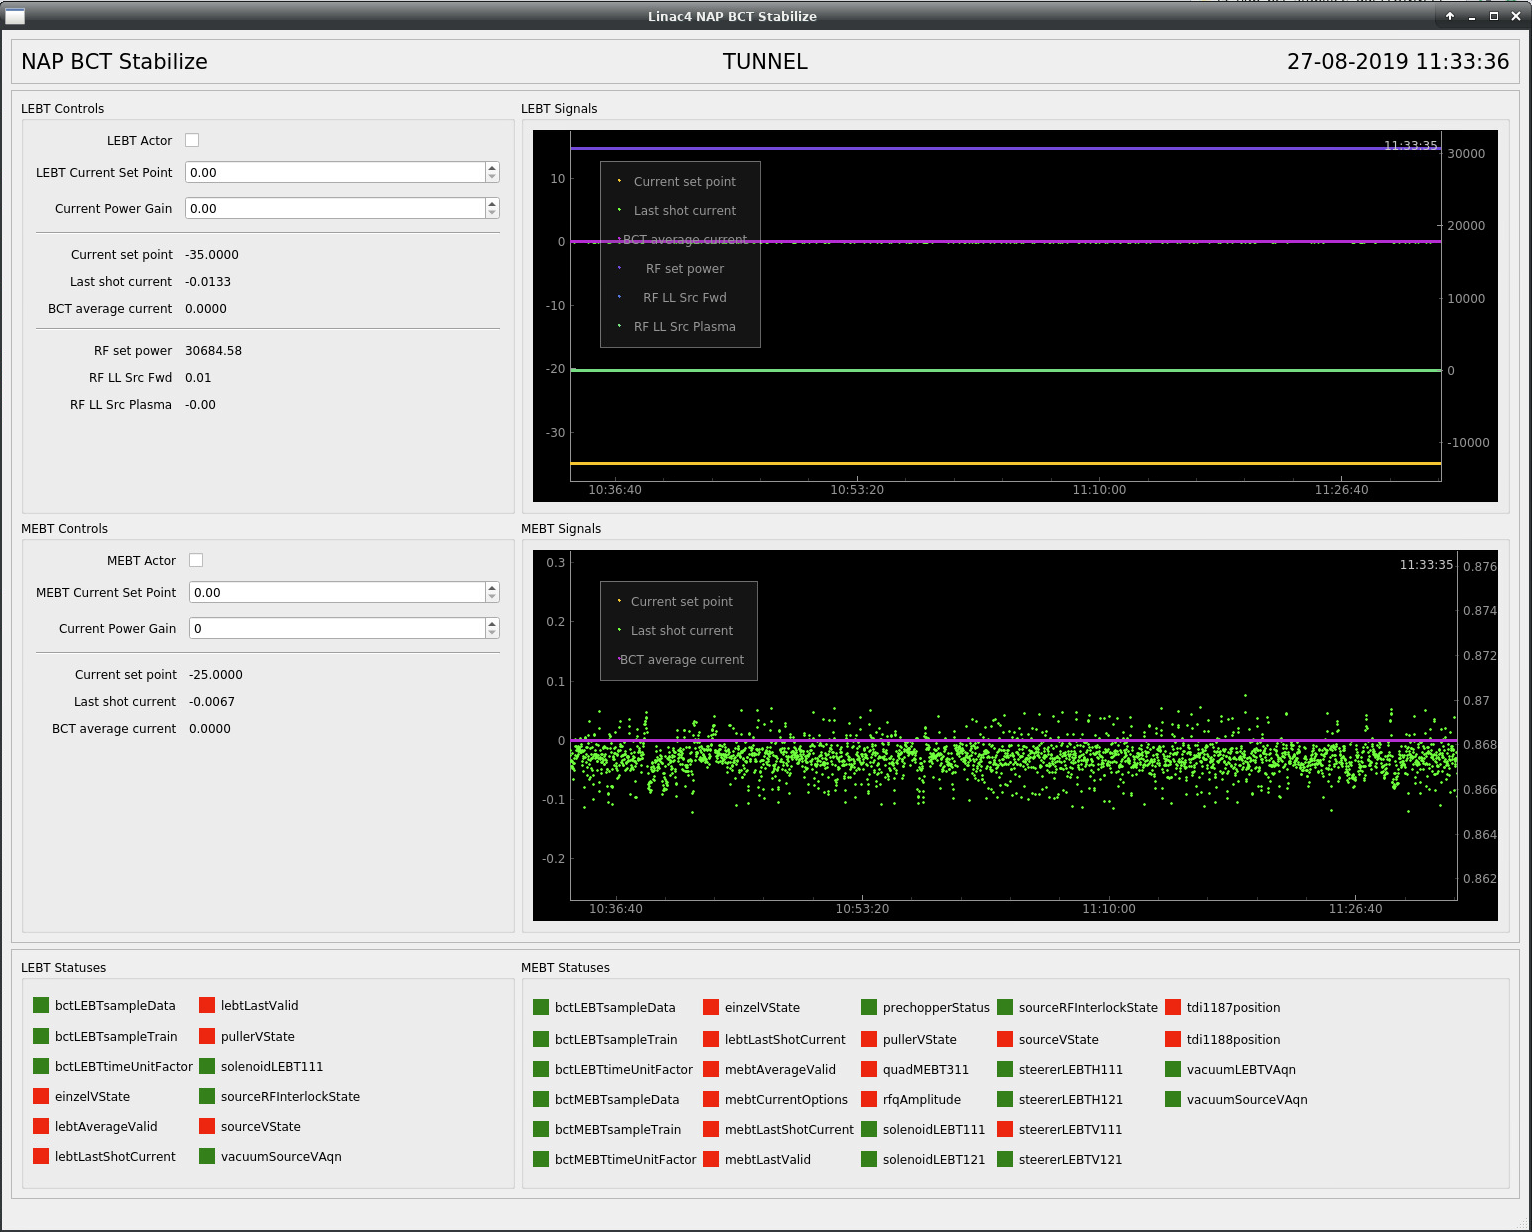
\includegraphics[width=14cm]{resources/img/Linac4SourceGui}
    \caption{Screenshot of the Linac4 Source Gui}
    \label{fig:linac4sourcegui}
\end{figure}

The Application where this Use Case is originated from is a \gls{gui} for the Linear Accelerator Linac4, whose tasks it is to boost negative hydrogen ions to high energies. The GUI will allow monitoring and manipulation of different device settings. Image \ref{fig:linac4sourcegui} shows a screenshot of an early version of the application. In the upper right part of the window are two graphs containing multiple scatter plots. Both graphs are implemented with the python graph library pyqtgraph, which we will explore in more detail in section \ref{sec:application:libraries:pyqtgraph}.
\cite{LinacFour,LinacFourGuiPres}


%% ==============================================
%%       Performance Metrics from Use Cases
%% ==============================================
\section{Performance Metrics from Use Cases}
\label{sec:usecases:metrics}

In this section we will collect metrics we can use to define a plotting libraries performance based on the insights we gained into the usage of these libraries from the use cases in this chapter. All of these Use Cases have in common, that they are displaying live data, which will be delivered with a certain frequency. If a plotting widget needs a very long time to redraw, this might result in updates piling up without the widget having time to redraw, if an update is always leading to a redraw. Long redraw cycles are not only a 
The most important metric we have to measure is without a doubt, how long the operations following a data update take. When collecting those times and calculating the average from it, we can make realistic predictions, if a widget will handle a certain update load under certain circumstances.

Even for applications containg graphs, which are not updated regularly, the time it takes the graph to redraw is very important for the interaction with the graphs, since it requires the graph to redraw as well. Slow redraw times will lead in these applications to stuttering use interfaces.

If a Use Case reveals a performance issue, it is important to investigate, where the source of the performance issue is rooted. Profiling is a very helpful procedure to decide, where improvements are needed most. A profile lists very detailed information about which functions consumed how much time in total, how often it has been called and how long a single call did take. With these informations, we can investigate, where we can change code to increase performance.

%% ==============================================
%%           Design and Implementation
%% ==============================================
%% Author: Fabian Sorn
%% ==============================================


\chapter{Design and Implementation of a Benchmark Framework}
\label{ch:application}

In this chapter, the findings from the previous chapters will be combined to
design and implement a benchmarking framework, which allows users to
benchmark specific charting operations. 


%% ==============================================
%%          Python Graph Libraries
%% ==============================================

\section{Python Graph Libraries} \label{sec:application:libraries}

When benchmarking different Python Graph libraries, we will focus our attention
on two popular contenders for the implementation, which are very well accepted
in the scientific community.

\subsection{Matplotlib} \label{sec:application:libraries:matplotlib}

Matplotlib is without a doubt the standard library for 2D data visualization in
Python. It offers publication quality visualization as well as an interactive
environment. The project was initialized by John D. Hunter as an easy to use
Python 2D plotting library, especially for users familiar with Data
Visualization in Matlab.
\cite{Matplotlib, MatplotlibHistory}

Matplotlib's central item is the \inlinecode{Python}{matplotlib.figure.Figure}.
The Figure itself does not yet display anything, neither a plot with axes nor
data. A plot is referred as an \inlinecode{Python}{matplotlib.axes.Axes}. A
figure can have multiple Axes in it. For each dimension in the data space the
Axes contains \inlinecode{Python}{matplotlib.axis.Axis} objects, which
represents the minimum and maximum data limit for each dimension of the data. An
Axes object can be personalized through axis labels and a title. In Matplotlib
terminology, Artists are everything which is visible in a Figure. This includes
Labels, Lines and Bar Graphs, Axis Items and more. The last crucial component is
the Canvas, which is not really a visual component in the plot, but the
component responsible for rendering the image. A summary of all components can
be seen in \ref{a:fig:matplotlib:content}

Matplotlib is built for many different use cases. While showing data in
\gls{gui} applications is one of them, other use cases, like generating plots as
images for publications are possible as well. This is achieved by Matplotlib's
different backends. All available Backends can be divided in interactive and
hard copy ones. An example for a interactive backend is in our case PyQt5, but
other Frameworks like Tkinter or PyGTK are supported as well. Non interactive
backends are for creating image files in different file formats like PNG, SVG,
PDF and more.
\cite{MatplotlibIntro, PythonDataVis}

Listing \ref{listing:application:matplotlib} shows the creation of a window
containing a plot representing a sinus curve through a line, a scatter plot and
a bar graph. For interaction, matplotlib offers a toolbar, which lets you select
between different interaction modes like panning and zooming. As a backend
Matplotlib's Qt5 backend was used.  The resulting window can be seen in
Screenshot \ref{a:fig:matplotlib:window}.

\lstinputlisting[ 
    caption=Definition of a Window containing a plot created with Matplotlib,
    language=python,
    label=listing:application:matplotlib,
    firstline=4,
    lastline=32
]{resources/code/matplotlib_demo.py}

\subsection{PyQtGraph} \label{sec:application:libraries:pyqtgraph}

PyQtGraph is a pure python plotting library. Even though it does not offer as
many features as other Python plotting libraries like Matplotlib, PyQtGraph
promises much better performance. The project was initialized by Luke Campagnola
and is focused on providing plotting functionalities for engineering and science
applications. It provides simple plots containing line graphs, scatter plots,
bar graphs and more, but also image and video displaying, Region of Interest
widgets, 3D visualization and more.  Since our benchmarking efforts will be
tightly focusing on the collected use cases, we will restrict our usage of its
features mainly on two dimensional plotting. PyQtGraph uses Qt's Graphics View
for drawing, which is a Framework for fast visualization of a large number of
custom 2D items. A big advantage it offers is a fast performance and the
possibility to interact and transform the scene through operations like
zooming or rotation.
\cite{GraphicsView}

Since PyQtGraph is built on top of Qt features, integrating it into Qt
applications is very simple. The central component for plotting is the
\inlinecode{Python}{pyqtgraph.PlotWidget}, which is derived from
\inlinecode{Python}{QtWidgets.QWidget}. When adding the plot widget to a
window, it comes with different components on the inside, as seen in
\ref{a:fig:pyqtgraph:content}. The central one is the
\inlinecode{Python}{pyqtgraph.PlotItem}, which is the actual plot. The widget
itself is only a wrapper for easy integration into Qt Applications. The plot
item contains different components of the plot, including a
\inlinecode{Python}{pyqtgraph.ViewBox}, the area data is visualized in,
a \inlinecode{Python}{pyqtgraph.AxisItem} representing the View Range
of the View Box, and a Title. Items which are actually representing a dataset are
added to the View Box. For this, PyQtGraph is offering different types of
representations like \inlinecode{Python}{pyqtgraph.PlotDataItem} for Scatter
Plots and Line Graphs and \inlinecode{Python}{pyqtgraph.BarGraphItem} for
representing data in a bar graphs.

Listing \ref{listing:application:pyqtgraph} shows the creation of a window
containing a plot representing a sinus curve in different ways. It displays the
same data sets in the same style as the Matplotlib example
\ref{sec:application:libraries:matplotlib}. The resulting window can be seen in
\ref{a:fig:pyqtgraph:window}.
\cite{PyQtGraphDoc}

\lstinputlisting[
    caption=Definition of a window containing a plot created with PyQtGraph,
    language=python,
    label=listing:application:pyqtgraph,
    firstline=2,
    lastline=25
]{resources/code/pyqtgraph_demo.py}


%% ==============================================
%%                   Analysis
%% ==============================================

\section{Analysis}
\label{sec:application:analysis}

After having a closer look at the two plotting libraries we will focus on, this
chapter will focus on the design of the benchmarking framework, which we can use
to investigate performance of both in the different use cases.

This section will focus on the conceptual design of such a framework, while the
following section \ref{sec:application:implementation} will focus on actual
implementation.

\subsection{Describing Performance of GUI systems}
\label{sec:application:analysis:performance}

From a Usability Engineering perspective, rendering performance is a vital
aspect, since it greatly impacts a \glspl{gui} response time. The general advice
on system's response times is 100 milliseconds, which is roughly the boundary
up to which a systems feels like it is instantly responding to input. Delays
over one second can already interrupt the thought process of the user, since he
is clearly noticing the delay. Delays over ten seconds on the other hand require
feedback from the system to signal the user it is performing long lasting tasks,
since the user often already wants to perform other tasks.
\cite{UsabilityEngineering}

An often used measurements for describing a system's rendering performance is the
frame rate, which describes the frequency, with which images appear on a screen.
This size originates from the movie industry, where the standard frame rate is 24
Frames per Second. The minimum frequency needed for the human eye to see a
consecutive movement from a sequence of images is as low as 16 Frames per
Second. This does not mean, that frame rates beyond this won't be recognized by
the human eye. Increasing the Frame Rate leads to the reduction of motion blur,
increasing details and clarity of a moving image.

Especially in the area of computer games, high frame rates are desirable, since
they will not only enhance the visual experience, but will give the player a
strategic advantage in a competitive environment.  A popular demonstration of
the increased clarity of high frame rates is the Blur Buster's UFO Motion Blur
Test website, which shows the same scene of fast moving cartoon UFO in different
frame rates (https://www.testufo.com).

In many Hardware Benchmarks, Frames per Second can be found as the central
description of a hardware component's abilities to render a complex scene. To
measure this, the hardware benchmark will try to rerender the scene as fast as
possible. At the same step in the rendering process of a single frame or image,
the current time stamp is recorded. From these series of timestamps we can
calculate the difference between two adjacent timestamps. This concept is known
as Delta Timing and gives us information, how long the rendering process is
taking us per Frame. In Video Games for example, this information allows us to
find out, how much an object in the displayed scene should have moved since the
last displayed frame. As a result, figure movement stays consistent, even under
different load scenarios.
\cite{DeltaTiming}

From the recorded timing information, we can calculate the frame rate $f$ from a
set of $m$ recorded time stamps $t_n$ as follows.
\cite{FrameRates}

$$f = \frac{1}{\frac{ \sum_{n=0}^{m-1} t_{n+1} - t_{n} }{ m - 1 }}$$

While frame rates already provides very important information from a user's
perspective, it does not yet help improving those from a developers perspective.
Profilers are software tools which are able to measure different aspects of
performance, like execution time, memory management, garbage collection and
more. The type of profiler we will mainly focus on is deterministic CPU
utilization profilers, collects information about time spent in functions, the
origin and amount of calls to these functions. With the help of this
information, optimization efforts can be directed to where they really can make
a difference. Additionally Profilers can not only uncover slow performing
functions, but also, if functions are more often called as intended by a programs
author.
\cite{CProfilerExample}

The standard option in Python to profile code, is the C extension cProfile,
which allows deterministic profiling of your Python programs. Compared to the
profiling profile, which is written in Python, cProfile offers a much lower
overhead, which makes it suitable for profiling longer running programs Compared
to the profiling profile, which is written in Python, cProfile offers a much
lower overhead, which makes it suitable for profiling longer running programs.
To provide this information about the execution of a program, cProfile does use
hooks for events, which are offered by the Python interpreter. These hooks are
callbacks, which allow cProfile to receive and record timing information about
every function executed by the Python interpreter. For profile and cProfile,
there are two limitations, which you have to be aware of when profiling
software.  The first one is the granularity of the underlying timer used for
recording the duration of an operation, which is mostly around 0.001 seconds.
The other limitation is the lag between the event being dispatched and the
profiler to get the current time. Since profiling is introducing a certain
overhead to the execution of a python program, it is not suitable for
benchmarking itself.
\cite{CProfiler}

\subsection{Use Cases}

\label{sec:application:analysis:usecase}

One important aspect of designing a framework, is the possible use cases it
offers to the user. Users interested in the performance of a graph library in a
specific scenario, have a clear idea of their use case. Most higher level
descriptions can be broken down in a simple operation or a sequence of
operations. Since these Use Cases are the central point of interaction with the
Framework, the we will define the following requirements, which have to be met
for the definition of Use Cases.

\begin{description}
    \item[Ease of Use] 
        The Framework should handle everything that is not relevant for the Use
        Case. The user should only define, what is part of the Use Case and
        nothing else.
    \item[Widget and Operation]
        The central items for defining a Use Case are a widget, and an operation
        which is executed on this widget.
    \item[Multiple Use Cases]
        Adding and removing Use Cases has to be possible without much effort.
    \item[Parameterization]
        A Use Case has to be reusable for different parameters and has to be
        easily extensible.
    \item[Performance Expectations]
        The author has to be able to define his performance expectations per use
        case.
    \item[Timeout]
        In case Use Cases take much longer than expect, it should be possible
        to define a timeout, which will terminate the Use Case execution, if
        reached.
\end{description}

One framework type, which allows a similar way of defining specific use cases,
are Testing Frameworks like unittest or pytest. Since most users are to an
extend familiar with their functionality, the interface should conform the
expectations built from the usage of these frameworks.

For easy execution of Use Cases, the Framework will offer a command line
interface, which offers similar functionality like other python tools. The
interface should conform the user's expectations in the same way with a few
additions specific for our needs. 

\begin{description}
    \item[Use Case Exection]
        Similar to Frameworks like pytest, it should be able to execute a full
        suite of Use Cases or only specific ones.
    \item[Meaningful Results]
        After execution, the user should be able to clearly see the results of
        his Use Cases. This includes the Use Case, its performance requirements,
        the actually achieved performance and the parameters used in the run.
    \item[Profiling]
        Since Profiling introduces additional overhead to the code's execution,
        profiling should be optional.
    \item[Profiling Visualization]
        Since profiles often contain large amount of data, they have to be
        visualized in a user friendly way.
\end{description}




%% ==============================================
%%                  Design
%% ==============================================

\section{Design}

\label{sec:application:design}

This section will focus on the design decisions for the framework and describing
the components involved. The most outer layer of the framework contains two
components. The first component is the command line interface, which offers the
user the possibility to execute his benchmarking use cases. Additionally the
interface offers functionality to display the results gathered by the framework.
The second component is the actual framework in the narrow sense, which is
responsible for providing the necessary interfaces for the definition of use
cases, the functionality for executing use cases, as well as recording the
performance metrics that are displayed later. We will refer to the executing
part of the framework as the launcher from now on.

\subsection{Benchmark Execution}

Figure \ref{fig:application:design:cli} shows the communication between the
user, the command line interface and the launcher for the application case of
executing a benchmarking use case from the command line.  When the User starts
the executable, a \gls{cli} instance is created, which parses the command line
arguments and instantiates the launcher. To keep the user interface
exchangeable, launcher and \gls{cli} are strictly separated from each other.
After the Launcher is initialized, it will import the use case modules. With the
completion of the step, the launcher can be started, which will execute all
collected use cases, collect the results and return them to the \gls{cli}, where
they can be displayed.

\begin{figure}[h]
    \centering
    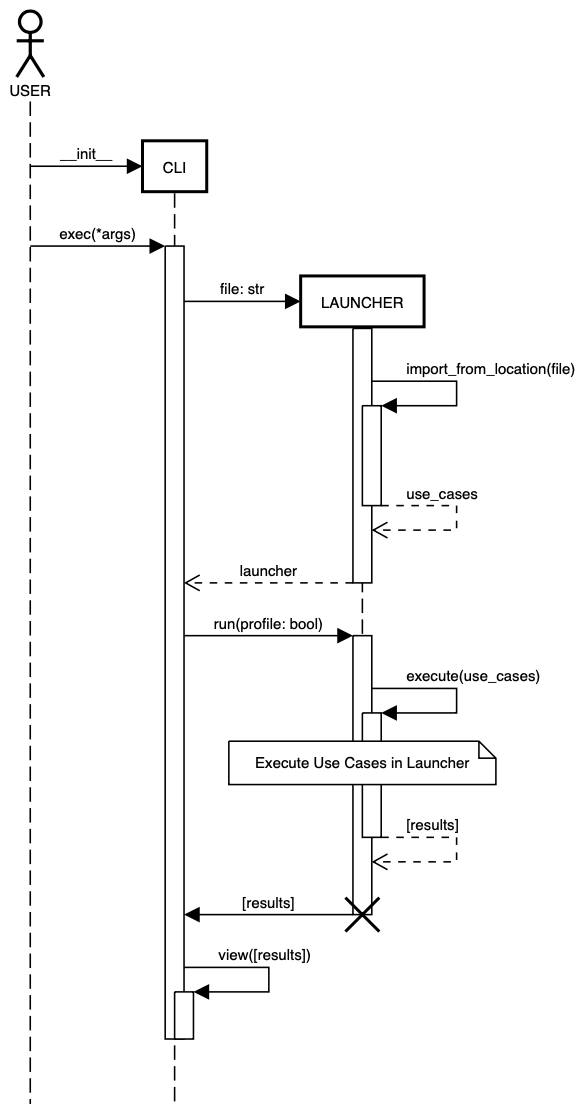
\includegraphics[width=11cm]{resources/img/sequence/cli}
    \caption{
        Sequence diagram showing the communication between the Command Line
        interface and the Framework.
    }
    \label{fig:application:design:cli}
\end{figure}

As next we will have a more detailed look at the execution of a collection of
use cases, which is visualized in depiction
\ref{fig:application:design:launcher}. We want to allow executing a whole suite
of use cases similar to testing frameworks allowing us to execute entire test
suites. This means that out launcher has to be able to handle multiple use
cases, execute them sequentially and save the record of each. Additionally, the
launcher has to be able to handle parameterized use cases and execute them for
every possible parameter combination similar to the parameterize functionalities
of many testing framework. 

For the execution we will introduce two new components to our framework. The
first component is the \gls{gui} window, which we will embed the widget in,
which we want to operate on. The second one is the executor, which is
responsible to execute the defined operation on the window and record timing
information and the profile. After our Launcher is initialized and out benchmark
files are properly imported, we will execute each use case in all possible
parameter combinations. For each Combination we create a benchmarking
window, which embeds the widget defined in the use case to display it. The
window will then be passed to the executor, which needs the window to execute
the operations defined in the use case on it. After the executor is fully
initialized, we can run it.

\begin{figure}[h]
    \centering
    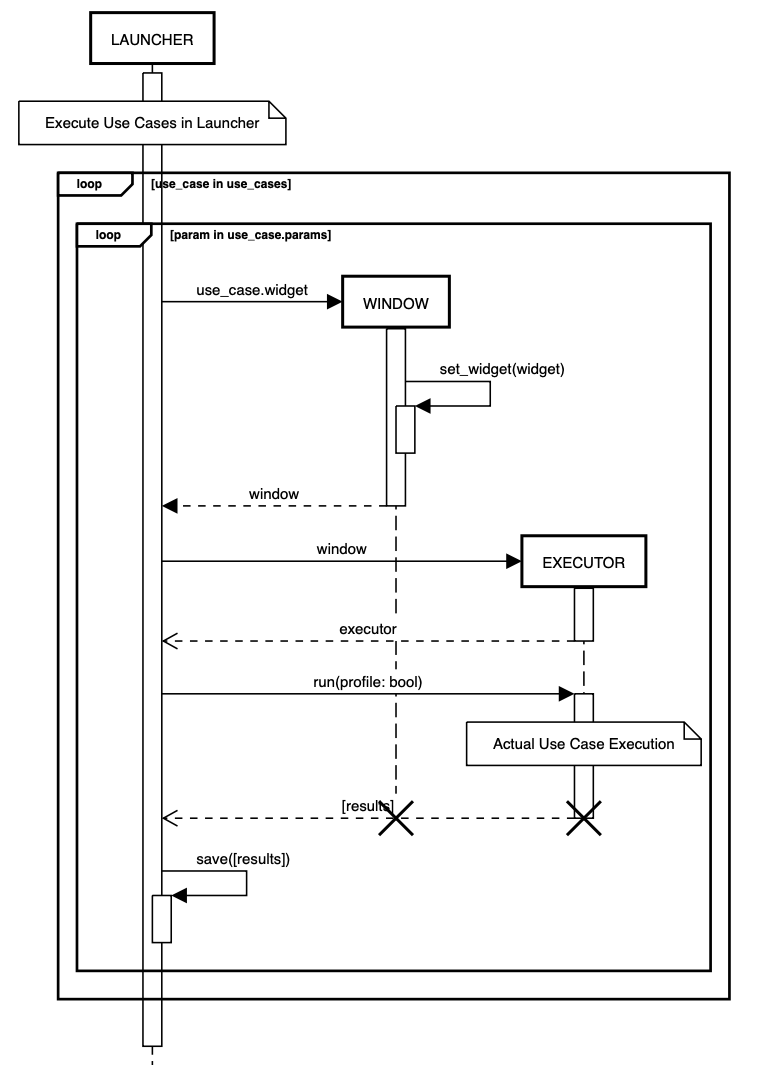
\includegraphics[width=12cm]{resources/img/sequence/launcher}
    \caption{
        Sequence diagram showing the creation of the benchmarking window and the
        executor.
    }
    \label{fig:application:design:launcher}
\end{figure}

Depiction \ref{fig:application:design:executor} shows this process in more
detail. Before each operation, the current time stamp is taken. If a profile is
supposed to be created, the profiler is started here as well. Afterwards the
operation, which we want to benchmark, is executed on the passed window
instance.  After it and all of its side effects are completed, the profiler is
stopped if necessary. This execution cycle is repeated, until the defined repeat
count or the timeout is reached. Afterwards, the timing information and the
profile data are can be returned to the launcher.

\begin{figure}[h]
    \centering
    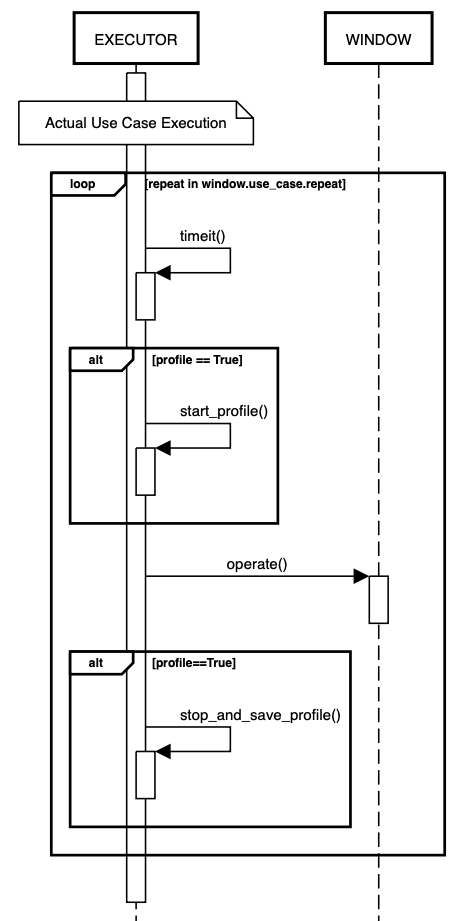
\includegraphics[width=8cm]{resources/img/sequence/executor}
    \caption{
        Sequence diagram showing the actual benchmarking execution on the window
        by the executor in more detail.
    }
    \label{fig:application:design:executor}
\end{figure}

Figure \ref{fig:application:design:classdiagram:widgetmark} shows the classes
from the prior sequence diagrams and their relations to each other. Since
Launcher and \gls{cli} are clearly separated from each other, it will be easily
possible to replace the User Interface without having to change any business
logic of the framework. 

\begin{figure}[h]
    \centering
    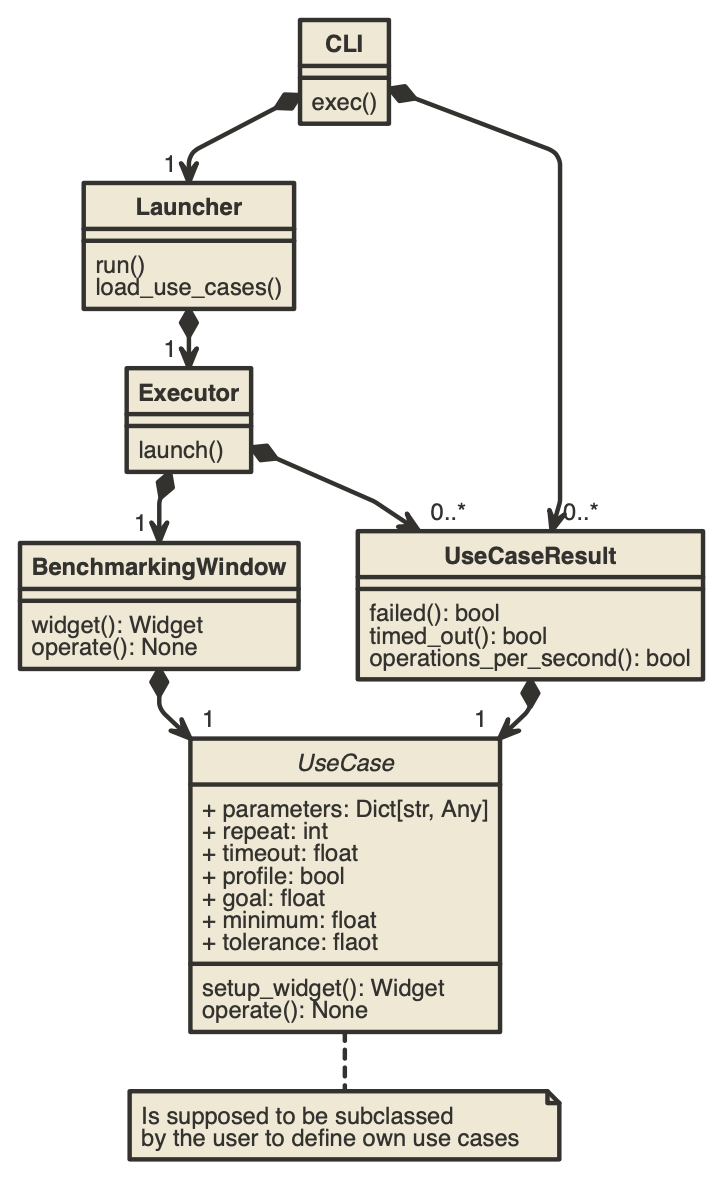
\includegraphics[width=8cm]{resources/img/class/widgetmark}
    \caption{
        Class diagram depicting all important classes involved in the
        Benchmarking Framework. 
    }
    \label{fig:application:design:classdiagram:widgetmark}
\end{figure}

\clearpage

\subsection{Use Case Definition}

\label{sec:application:design:usecases}

In this section we will have a closer look at the design of Use Case definition
after collecting the requirements for Use Cases in section
\ref{sec:application:analysis:usecase}. To define a Use Case, Users will have to
define a class in a python module. To mark the class as a Use Case, it will have
to subclass the class \inlinecode{Python}{UseCase}. This will allow us to have a
clearly defined interface for Use Cases, and makes the discovery of use case
classes easier on execution. Figure
\ref{fig:application:design:classdiagram:widgetmark} shows the classes methods.

To define plotting benchmarks that are executable with different plotting
libraries we will implement a unified interface for them, that can be
implemented using different graph libraries. For now we will limit this
interface to the functionality of our use cases we need. Such an interface is of
course limited as well to the functionality that all libraries used for the
implementation offer in common. With using the parameterization functionalities
of our Use Cases, we can simply define higher level plotting benchmarks and
execute them using different libraries to compare the results from each library.

\begin{figure}[h]
    \centering
    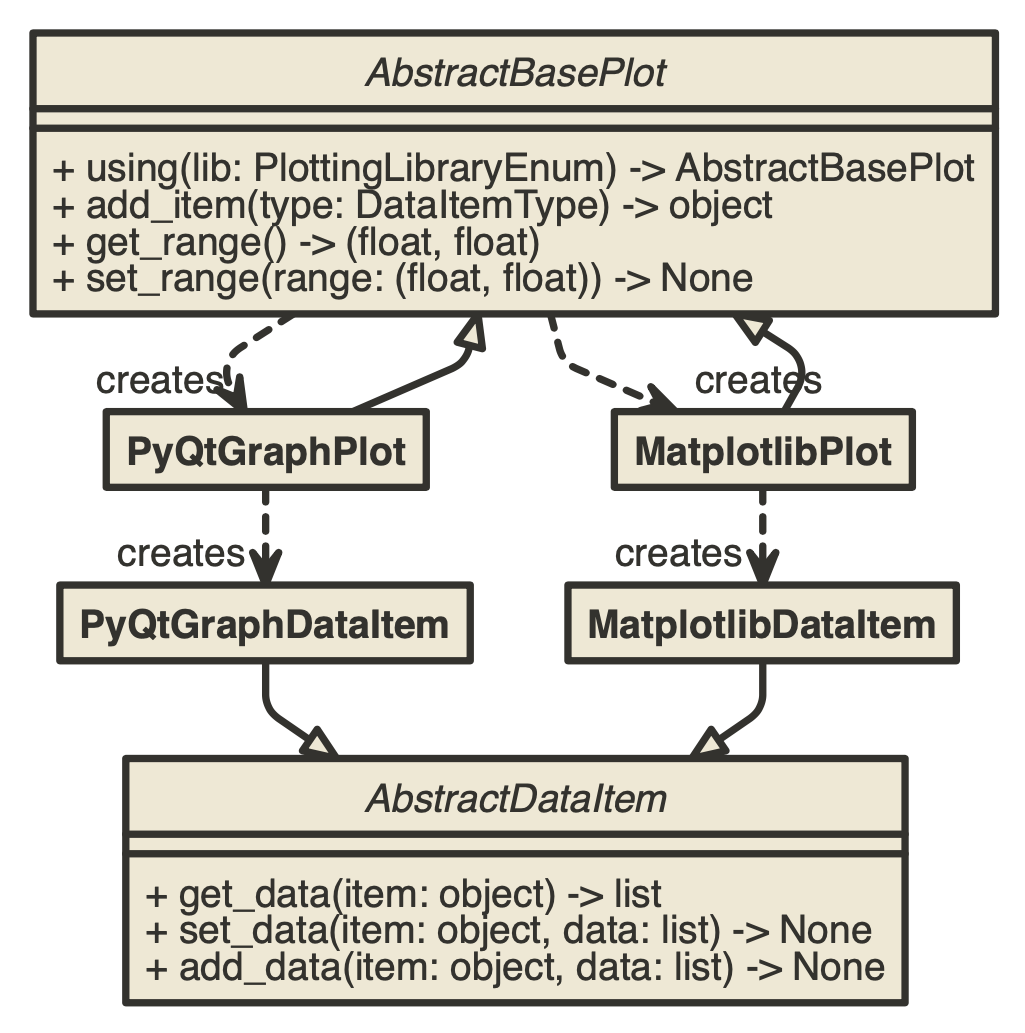
\includegraphics[width=7cm]{resources/img/class/plotabstraction}
    \caption{
        Class diagram depicting the plot abstraction interface and two
        subclasses for the python plotting libraries PyQtGraph and Matplotlib. 
    }
    \label{fig:application:design:classdiagram:plot}
\end{figure}

Figure \ref{fig:application:design:classdiagram:plot} shows the abstract
base classes for the plot widget as well as data items like curves, bar graphs,
scatter plots and more. The class \inlinecode{Python}{AbstractBasePlot} offers
plot functionalities to add a new item, get the current view range, set the
current view range and a factory method for creating a plot using a specific
plotting library. The two subclasses \inlinecode{Python}{PyQtGraphPlot} and
\inlinecode{Python}{MatplotlibPlot} can implement the functionality defined by
the base class using the specific libraries \gls{api}. The
\inlinecode{Python}{AbstractDataItem} on the other hand defines a common
interface for setting, getting and adding new data to a data item of a plot.
Similar to the plot, the two subclasses \inlinecode{Python}{PyQtGraphDataItem}
and \inlinecode{Python}{MatplotlibDataItem} implement this.

Code Example \ref{listing:application:plotabstraction} shows an example of the
interface usage in a standard Qt window. Which library is used for the
visualization can be simply controlled by choosing it during the widget's
creation using the \inlinecode{Python}{AbstractBasePlot} factory method.

\lstinputlisting[ 
    caption=Creating a plot showing a sinus curve using the Plot Abtraction 
            Layer,
    language=python,
    label=listing:application:plotabstraction,
    firstline=9,
    lastline=30
]{resources/code/plot_abstraction.py}


\subsection{User Interface}

In this section we will have a look at the design of the command line interface
of the framework based on the requirements we collected in
\ref{sec:application:analysis:usecase}. Since our command line is supposed to be
easily usable for users of other testing frameworks, our command line interface
should be kept similar. Listing \ref{listing:application:cliusage:location}
shows how to specify the location of one or multiple use cases from the command
line. We will use a specific naming convention to mark files who define use
cases. Each file which is supposed to be searched has to start with the prefix
\inlinecode{bash}{bench_*}. This pattern should be configurable from the command
line as well.

\lstinputlisting[ 
    caption=Starting benchmarks from the command line,
    language=bash,
    label=listing:application:cliusage:location,
    lastline=39
]{resources/code/widgetmark_cli_usage.sh}

Additionally the command line should allow us to configure, if we want to run
the framework with or without profiling, as well as the location the files are
saved in. Listing \ref{listing:application:cliusage:profile} shows these
configuration options on the command line as well as the generated files.

\lstinputlisting[ 
    caption=Starting benchmarks and create profiles for them,
    language=bash,
    label=listing:application:cliusage:profile,
    firstline=40,
    lastline=52
]{resources/code/widgetmark_cli_usage.sh}

Additionally the \gls{cli} should provide a visualization option for these binary
profile files, which listing \ref{listing:application:cliusage:visualize} is
showing. Simply printing profile files would not be very helpful, since they can
grow very fast in size. Because of this, there are multiple tools available,
which offer a much more user friendly visualization. For our purposes we decide
for \emph{snakeviz}, a browser based graphical viewer for profile files.
\cite{Snakeviz}

To improve the usability of the \gls{cli}, a help function should be offered which
explains what the framework is and how it is going to be used.
Listing \ref{listing:application:cliusage:help} shows how such a help message
could look like. Additionally it should be possible to run the \cls{cli} with
additional output when searching for the cause of bugs. 

\lstinputlisting[ 
    caption=Starting benchmarks and create profiles for them,
    language=bash,
    label=listing:application:cliusage:help,
    firstline=58,
    lastline=68
]{resources/code/widgetmark_cli_usage.sh}

The \cls{cli} output should contain all important information about the found files,
the use cases, the performance requirements, the parameters and the actual
reached frame rate. Listing \ref{listing:application:cliusage:output} shows these
informations on the command line after all found benchmarks were executed.

\lstinputlisting[ 
    caption=Output of the CLI with showing the benchmark results,
    language=bash,
    label=listing:application:cliusage:output,
    firstline=69,
]{resources/code/widgetmark_cli_usage.sh}




%% ==============================================
%%             Implementation
%% ==============================================

\section{Implementation} \label{sec:application:implementation}

This section will focus on the actual implementation of the framework based on
the Analysis from section \ref{sec:application:analysis}, the design from
section \ref{sec:application:design} and the Use Cases from chapter
\ref{ch:usecases}. As a name we choose \emph{widgetmark}, a composite of widget
and benchmark.  The language we use is Python in the version 3.6 to use newer
language features like typing hint, which will highly improve the usability of
the framework.

\subsection{Project Structure}

The first part of the implementation is setting up our project in Python, which
figure \ref{fig:application:implementation:structure} is showing. The project
will follow python best practices with a package \emph{widgetmark} for the
source code and \emph{tests} for unit tests. Additionally the project contains
the two generated files \emph{\_version.py} and \emph{versioneer.py} for getting
version information from version control tags, \emph{README.md} for a
introduction into the project, \emph{setup.cfg} for tooling configuration and
\emph{setup.py} for dependency definition and installation instructions.

\begin{figure}[h]
    \centering
    \framebox[\textwidth]{%
        \begin{minipage}{0.9\textwidth}
            \dirtree{%
                .1 project.
                .2 widgetmark.
                    .3 base.
                        .4 benchmark.py.
                        .4 executor.py.
                        .4 launcher.py.
                    .3 qt.
                        .4 benchmark.py.
                        .4 executor.py.
                        .4 plot.py.
                        .4 util.py.
                    .3 cli.
                        .4 \_\_main\_\_.py.
                        .4 cli.py.
                        .4 cli\_view.py.
                        .4 loader.py.
                    .3 \_version.py.
                .2 tests.
                    .3 \_\_init\_\_.py.
                    .3 \dots.
                .2 setup.py.
                .2 setup.cfg.
                .2 versioneer.py.
                .2 README.md.
            }
        \end{minipage}
    }
    \caption{Widgetmark project structure}
    \label{fig:application:implementation:structure}
\end{figure}

\subsection{Subpackage widgetmark.base}

The first sub-package of our implementation is the package
\inlinecode{Python}{widgetmark.base}. In this package we will define all base
classes for our benchmarking framework, which are not part of the user
interface. To keep the framework extensible and not limited to Qt as its
\gls{gui} framework, we will skip qt specific implementations of functionality
in this package and only offer common functionality not related to \gls{gui}
operations. Qt specific implementations will be part of the
\inlinecode{Python}{widgetmark.qt} package.

\subsubsection*{benchmark.py}

The first class for our implementation is the use case interface. Python does
not support interfaces, but offers abstract classes we can use to define our
interface by simply not provide any implementations for functions.

\lstinputlisting[ 
    language=Python,
    linerange={2-2, 14-14}
]{resources/widgetmark/base/benchmark.py}

When distinguish three different types of information that can be
defined in a use case: functions all subclasses have to implement, attributes
subclasses have to implement and attributes subclasses can implement.
Mandatory functions can be simply implemented as abstract methods using the
\inlinecode{Python}{abstractmethod} decorator provided by the
\inlinecode{Python}{abc} package.

\lstinputlisting[ 
    language=Python,
    linerange={116-117, 124-124}
]{resources/widgetmark/base/benchmark.py}

Non mandatory attributes can be easily implemented as class attributes.

\lstinputlisting[ 
    language=Python,
    linerange={30-30}
]{resources/widgetmark/base/benchmark.py}

For implementing mandatory attributes, \inlinecode{Python}{abc} does not offer
any standard decorators, but we can use \inlinecode{Python}{property} in
combination with the \inlinecode{Python}{abstractmethod} decorator to create
abstract properties for out class. While such an implementation does not
actually depict a mandatory attribute on a class level, the abstract property
can be implemented as a class attribute in subclasses.

\lstinputlisting[ 
    language=Python,
    linerange={56-58, 64-64}
]{resources/widgetmark/base/benchmark.py}

\lstinputlisting[ 
    language=Python,
    linerange={19-19, 22-22}
]{resources/widgetmark/bench_label.py}

With this implementation, there is no visual difference between defining
mandatory or optional attributes in use case classes, but we can enforce, that
all all mandatory attributes have been implemented. Both, class attributes and
abstract properties can also be accessed the same way after the class is
initialized using \inlinecode{Python}{instance.attribute}.

The next class defined in this module is the \inlinecode{Python}{UseCaseResult}
class, which is based on a single use case. For parameterized use cases, there
will be a result instance for each parameter combination. The result object
should comprise all information we have recorded from the use case. To make sure
that use cases are read only after their initialization, we hold the information
in private instance attributes and allow reading access only over properties
without defining property setters. Additionally we offer convenient properties
for checks on the results. An example is a \inlinecode{Python}{failed} property
that can be used to check for exceptions instead of comparing the
\inlinecode{Python}{result.exception is None} property against
\inlinecode{Python}{result.failed}.

\lstinputlisting[ 
    language=Python,
    linerange={173-180, 194-198, 245-246, 248-248}
]{resources/widgetmark/base/benchmark.py}

The last class defined in the module is the benchmarking window, which
incorporates the widget defined in the use case and grants access to the
operation we want to benchmark. Wrapping the operation allows us to access it
later in the executor without having to keep a direct reference to the use case.
Since our goal is to keep the base implementation free from \gls{gui} framework
specific functionality, we won't subclass any Qt window classes like
\inlinecode{Python}{QtWidgets.QMainWindow}.

\subsubsection*{executor.py}

The executor module contains the class
\inlinecode{Python}{AbstractBaseExecutor}, which is responsible for executing
the benchmarking operations on the window, record the results and create a
fitting instance of the \inlinecode{Python}{UseCaseResult} class.

As \ref{fig:application:design:executor} shows, for recording execution times,
we need a loop like execution of the same operation over and over again. Simply
using a loop can lead to unrealistic results, since we have to give back the
control to the control loop in between operations to not skip on pending work
caused by our operation. The practical implementation of this is dependent on
the used \gls{gui} framework and will not be part of this class. As for the
benchmarking window, this implementation will be done in a fitting executor
subclass in package \inlinecode{Python}{widgetmark.qt}.

For all \gls{gui} independent functionalities, this class does provide
implementations. As seen in \ref{fig:application:design:executor} an executor
instance is initialized for every parameter combination of every use case. After
the initialization, a window can be attached to the executor through
\inlinecode{Python}{set_window()}. The execution can then be launched using the
\inlinecode{Python}{launch()} method. 

\lstinputlisting[
    language=Python,
    linerange={38-56}
]{resources/widgetmark/base/executor.py}

Internally the abstract protected function \inlinecode{Python}{_launch()} is
called, which gives \gls{gui} specific subclasses an opportunity to set up the
actual execution loop. This loop can use the protected operation
\inlinecode{Python}{_redraw_operation}, which is responsible for calling the
operation on the window, collect timing information and control the profiler.

\lstinputlisting[
    language=Python,
    linerange={107-121}
]{resources/widgetmark/base/executor.py}

For recording the current time-stamp we can use the \inlinecode{Python}{time()}
function of the python package \inlincode{Python}{time}, which returns us the
current time as floating point number. From this time-stamp and the last
recorded one we can calculate the delta timing for the last step. The current
time will be saved in an instance attribute for the next operate.

\lstinputlisting[
    language=Python,
    linerange={154-159}
]{resources/widgetmark/base/executor.py}

The protected function \inlinecode{Python}{_profile} is responsible for
controlling the profiler, which is used to profile the use case operation and
combine the profiling stats from each step to a single profiling stat. Before
the old step the current Profile will be disabled, the stats are added to the
previously saved ones and the new profile will be enabled.

\lstinputlisting[
    language=Python,
    linerange={124-137}
]{resources/widgetmark/base/executor.py}

The last important function is \inlinecode{Python}{_check_if_completed()}
function, which stops execution if either the timeout or the repeat counter of
the use case is reached. If one is the case, the protected function
\inlinecode{Python}{_complete()} is called. Since reaching the end of the
execution cycle means stopping the execution loop, this step is \gls{gui}
framework specific and will be implemented in the subclasses. 

\lstinputlisting[
    language=Python,
    linerange={139-152}
]{resources/widgetmark/base/executor.py}

\subsubsection*{launcher.py}

The module \inlinecode{Python}{launcher} contains the class
\inlinecode{Python}{Launcher}. As figure \ref{fig:application:design:launcher}
shows, the purpose of the Launcher class is to create fitting benchmarking
windows and executors for the use cases it was passed on initialization. The
launcher can be initialized using either a list of types, which are derived from
the \inlinecode{Python}{UseCase} class or with a list of file locations, where
these classes are defined. If a list of files is passed, the fitting classes are
imported using the \inlinecode{Python}{importlib} module which python offers.
To make sure we import only classes that we want, we filter the found classes by
their name and their type. The filtering by name is for cases the user specifies
a specific name or name pattern on the command line, the type filtering is for
not accidentally trying to initialize classes which do not define use cases.
This way use case files can safely contain other class definitions without
leading to errors.

\lstinputlisting[
    language=Python,
    linerange={123-126, 133-154}
]{resources/widgetmark/base/launcher.py}

The initialized launcher instance can be started using the
\inlinecode{Python}{run()} method, which takes a parameter
\inlinecode{Python}{profile} for controlling if the executor will create a
profile of the use case or not. Before initializing window and executor we
create a list of all parameter combinations. For each of these parameter
combinations we initialize the use case class. To grant access in the use case
class to these parameters, we set them as instance attributes to the initialized
use case instance. If the use case class defines for example the parameters
\inlinecode{Python}{'number': [0, 1]}, we can access the value of this
parameter in the use case class during execution by calling 
\inlinecode{Python}{self.number}.

\lstinputlisting[
    language=Python,
    linerange={90-119}
]{resources/widgetmark/base/launcher.py}

To resolve the right window and executor implementation for the backend defined
by the use case, we have the class \inlinecode{Python}{BackendResolver} which
does iterates through a classes subclass using the underscore function
\inlinecode{Python}{__subclasses__()} to find one fitting to the requested
backend. For this each subclass defines a class attribute
\inlinecode{Python}{gui_backend}, which can be compared to the
\inlinecode{Python}{backend} class attribute of the use case classes.

\subsection{Subpackage widgetmark.qt}

This package contains qt specific implementations of the benchmarking window and
the executor, as well as the qt plotting interface.

\subsubsection*{benchmark.py}

This module provides a Qt based implementation of the
\inlinecode{Python}{AbstractBenchmarkingWindow} based on 
\inlinecode{Python}{QtWidgets.QMainWindow}. Since Python supports multi
inheritance, the Qt benchmarking window can be implemented as follows. The
\inlinecode{Python}{make_qt_abc_meta()} function in this class definition is for
solving the meta class conflict between qt classes and the
\inlinecode{Python}{ABCMeta} from the \inlinecode{Python}{abc} package. This is
achieved by returning a metaclass that is derived from both the meta class of
\inlinecode{Python}{QMainWindow} and \inlinecode{Python}{ABCMeta}. Its
implementation can be found in the \inlinecode{Python}{util.py} module of the
same package.

\lstinputlisting[
    language=Python,
    linerange={7-9}
]{resources/widgetmark/qt/benchmark.py}

\subsubsection*{executor.py}

This module provides a Qt based implementation of the
\inlinecode{Python}{AbstractBenchmarkExecutor} based on
\inlinecode{Python}{QtCore.QObject}. The executor has to start a Qt application
and implement two functions based on it: \inlinecode{Python}{_launch()} and
\inlinecode{Python}{_complete()}. Initialization of the benchmark execution loop is the
purpose of \inlinecode{Python}{_launch}. To make sure, that no pending events
are skipped, we want to give back control to Qt's event loop after each time our
operation we want to benchmark is executed. In Qt we can achieve such a loop
by using the \inlinecode{Python}{QtCore.QTimer} with a timeout of zero seconds.
Such a timer will timeout every time it is possible. 
\cite{QTimer}

To the timer's timeout signal we can connect the executor's base's
\inlinecode{Python}{_redraw_operation} function, which handles profiling, timing
and operation execution. After the timer is set up we can start the event loop
of our Qt application.

\lstinputlisting[
    language=Python,
    linerange={60-64}
]{resources/widgetmark/qt/executor.py}

After the executor's base notices in its
\inlinecode{Python}{_check_if_completed} function, that either the timeout or
the maximum repeat counter is reached, it will call the
\inlinecode{Python}{_complete} function. Its purpose is not only to wrap the
recorded performance figures in a \inlinecode{Python}{UseCaseResult} instance,
but also to stop the execution loop. Since the loop is based on a
\inlinecode{Python}{QtCore.QTimer}, we can use its \inlinecode{Python}{stop()}
function to achieve this.

\lstinputlisting[
    language=Python,
    linerange={66-77}
]{resources/widgetmark/qt/executor.py}

The Executor is also responsible to start and quit the
\inlinecode{Python}{QtWidgets.QApplication}. One caveat worth mentioning in this
context is, that there should only be a single instance of the application
running, since multiple \inlinecode{Python}{QApplication} instances will lead to
problems. Because of this, the executor class has to make sure, that there is
no existing one before creating a new one.

\lstinputlisting[
    language=Python,
    linerange={79-87}
]{resources/widgetmark/qt/executor.py}

Since the window and the widget is exposed during the benchmark execution, the
user is able to interact with it. Since these interactions are not part of the
use case, they would affect the results negatively, since their work effort
would be counted as work produced by the use case. Because of this, we have to
filter out all operations, which are not directly caused by operations of the
use case. As described in section \ref{sec:fundamentals:qt:eventloop}, Qt offers
us the possibility to install event filters, which can filter out all events
coming from the window system. For our purposes we want to filter out all mouse
interactions using the following class derived from
\inlinecode{Python}{QtCore.QObject}.

\lstinputlisting[
    language=Python,
    linerange={9-10, 15-27, 29-32}
]{resources/widgetmark/qt/executor.py}

\subsubsection*{plot.py}

The module \inlinecode{Python}{widgetmark.qt.plot} contains the implementation
of the abstraction layer for plotting operations.  As described in section
\ref{sec:application:design:usecases} and in figure
\ref{fig:application:design:classdiagram:plot}, we want to introduce an
abstraction layer for the plotting libraries we are focusing on to write
benchmark use cases that are reusable for multiple plotting libraries.  This
abstraction layer should allow us to perform common actions on different
plotting libraries without relying on their library specific \gls{api}. The
abstraction layer itself is implemented as an abstract class, that provides a
factory method which returns the fitting subclass to the passed plotting
library.

\lstinputlisting[
    language=Python,
    linerange={44-48, 54-57, 60-63, 70-76, 87-97}
]{resources/widgetmark/qt/plot.py}

Each operation we want to use will get its own method in this abstract class. As
an example we will have a look at the \inlinecode{Python}{add_item} function,
which allows us to add a new item to the plot, which displays some data.

\lstinputlisting[
    language=Python,
    linerange={107-108, 118-118}
]{resources/widgetmark/qt/plot.py}

For PyQtGraph we can implement the \inlinecode{Python}{add_item} function based
on the \inlinecode{Python}{PlotDataItem}.

\lstinputlisting[
    language=Python,
    linerange={186-187, 189-196, 201-209}
]{resources/widgetmark/qt/plot.py}

For Matplotlib on the other hand we can use the \inlinecode{Python}{Line2D}
object for implementing the same function.

\lstinputlisting[
    language=Python,
    linerange={247-263, 279-289}
]{resources/widgetmark/qt/plot.py}

Both functions will return objects derived from the same
\inlinecode{Python}{AbstractDataItem}, which allows reading, writing and adding
data in form of a two dimensional numpy array containing x and y-values, which
fits our planned usage in listing \ref{listing:application:plotabstraction}. In
our use cases, we can add the plotting library we want to benchmark as a
parameter in its \inlinecode{Python}{parameters} section which we can then pass
to the factory function \inlinecode{Python}{using()} of the
\inlinecode{Python}{AbstractBasePlot} class. This way we can benchmark the exact
same use case in two completely different plotting libraries without having to
define two separate use cases.

\subsection{Subpackage widgetmark.cli}

The last package of our project's source code contains all modules related to
the command line interface. It's purpose is accept user input to start the
launcher with the files or use cases the user want as well as to present the
results gathered from execution. Additionally it write the recorded profiles to
separate files to a location defined by the user and start the visualization for
them using the \inlinecode{Python}{snakeviz} python application. For defining
command line arguments, the python package \inlinecode{Python}{argsparse} is
used, which allows convenient parsing of arguments passed on the command line
when executing the \gls{cli} module from the command line. Additionally, a help
option will be added, which explains the usage when the user executes
\inlinecode{bash}{widgetmark --help}.

When installing \inlinecode{Python}{widgetmark} using
\inlinecode{Python}{setuptools}, we can register wrap register our \gls{cli} as
an console script. This allows us to make a Python function accessible from the
command line. In the module main, we have our central main method, which
initializes the \gls{cli} and executes it.

\lstinputlisting[
    language=Python,
    linerange={4-6}
]{resources/widgetmark/cli/__main__.py}

In the module \inlinecode{bash}{setup.py} we can register this function as
a \inlinecode{Python}{console_script} follows and define the name of the
produces executable. In our case this will simply be
\inlinecode{Python}{'widgetmark'}

\lstinputlisting[
    language=Python,
    linerange={65-66, 77-79, 99-99}
]{resources/widgetmark/setup.py}




%% ==============================================
%%          Use Case Implementation
%% ==============================================

\section{Use Case Implementation}

This section will focus on the implementation of the use cases described in
chapter \ref{ch:usecases} based on the WidgetMark framework and its plotting
library abstraction classes. The use cases will be parameterized to use
Matplotlib as well as PyQtGraph for the evaluation.


%% LaTeX2e class for student theses
%% sections/content.tex
%%
%% Karlsruhe University of Applied Sciences
%% Faculty of  Computer Science and Business Information Systems
%% Distributed Systems (vsys)
%%
%% Prof. Dr. Christian Zirpins
%% christian.zirpins@hs-karlsruhe.de
%%
%%
%% Version 0.2, 2017-11-15
%%
%% --------------------------------------------------------
%% | Derived from sdqthesis by Erik Burger burger@kit.edu |
%% --------------------------------------------------------


\chapter{Performance optimization}
\label{ch:optimization}

\section{Optimizing line graph performance}
\label{sec:optimization:lines}

%% ------------------------------------------------------------
%% \subsection{Optimize the amount of rendering calls}
%% \label{sec:optimization:lines:rendercalls}

%% \dots

%% ------------------------------------------------------------
\subsection{GPU accellerated Rendering}
\label{sec:optimization:lines:opengl}

\dots

%% ------------------------------------------------------------
\section{Optimizing scatter plot performance}
\label{sec:optimization:SecondSection}

\subsection{Incremental data updates}

\dots

%% ==============================================
%%                   Evaluation
%% ==============================================
%% Author: Fabian Sorn
%% ==============================================

\chapter{Evaluation}
\label{ch:evaluation}

In this chapter we will evaluate the framework we designed and developed in the
last two chapters. We will start by evaluating, if the implementation fits our
requirements, by implementing the use cases presented in chapter
\ref{ch:usecases} and investigating their results. This will be followed by an
evaluation of the performance overhead the framework is producing, by comparing
the results with a minimal PyQt application recreating the same use case.

%% ==============================================
%%          Use Case Implementation
%% ==============================================

\section{Use Case Implementation}

This section will focus on the implementation of the use cases described in
chapter \ref{ch:usecases} based on widgetmark and its plotting library
abstraction layer. To have an overview of the development of the performance
of each use case depending the increasing plot counts, curve counts or dataset
sizes, we will run each use case with different parameters. We will start with
smaller sizes and increase them until we reach the use cases demanded
requirements. As a minimum refresh rate we will take the update frequency of the
use case. We will set the goal frame rate to 60Hz, which matches most modern
monitors. As data we will take random points each redraw, so we can be sure that
we will get a full redraw every time. As a repeat count we will take a
reasonable big number of 2000 redraws. Additionally we will define a timeout
that can stop use cases which take an unexpected long amount of time. Each use
case will be tested against both PyQtGraph and Matplotlib.

All of our three use cases have a very common setup. To avoid duplicated code,
we will define a setup helper class next to the use cases, which each one can
take advantage of. The implementation of its widget setup function can be seen
in listing \ref{listing:application:usecases:helper}. This helper function is
responsible for initializing a given number of plots, curves and random data
sets.

\lstinputlisting[ 
    caption=Setup helper function for creating plots, visualization items and
    data sets,
    language=python,
    label=listing:application:usecases:helper,
    linerange={20-27, 43-57}
]{resources/widgetmark/benchCern.py}

\subsection{Distributed Oscilloscope for BE-CO-HT}

The Distributed Oscilloscope features a central plot containing up to 8 curves
displaying up to 100,000 points at a time. To handle the update frequency of 25
Hertz, we will need a minimum frame rate of 25 frames per second. Listing
\ref{listing:application:usecases:ht:params} shows the implementation of these
parameters in a use case class as class attributes.

\lstinputlisting[ 
    caption=Definition of the parameters for the BE-CO-HT use case.,
    language=python,
    label=listing:application:usecases:ht:params,
    linerange={73-74, 79-89}
]{resources/widgetmark/benchCern.py}

Listing \ref{listing:application:usecases:ht:methods} shows the implementation
of the widget setup and the operation. For the setup we use the helper function
defined in listing \ref{listing:application:usecases:helper}. Since we only
create a single plot, we return it as the widget to use. The next function is
our operation definition, where we choose data and display in in our created
plots. To choose data from our random data sets, we take the current redraw run
as an index, which can be accessed through the runtime context object, that
every use case has access to.

\lstinputlisting[ 
    caption=Widget setup and operation definition for the BE-CO-HT use case.,
    language=python,
    label=listing:application:usecases:ht:methods,
    linerange={91-106}
]{resources/widgetmark/benchCern.py}

\subsection{Monitoring Application for BE-OP-LHC}

Our second use case features one central plot containing up to 3000 curves
displaying up to 2 * 3600 points, which should be updated every second. Listing
\ref{listing:application:usecases:ht:params} shows the implementation of these
requirements as parameters in the use case class. Widget Setup and operation
definition do not differ from listing
\ref{listing:application:usecases:ht:methods}.

\lstinputlisting[ 
    caption=Definition of the parameters for the BE-OP-LHC use case.,
    language=python,
    label=listing:application:usecases:ht:params,
    linerange={109-110, 115-125}
]{resources/widgetmark/benchCern.py}

\subsection{Linac4 Source GUI for BE-CO-APS}

Compared to the prior two use cases, this use case features multiple plots,
which means we can extend our parameter list with another entry for the plot
count. The implementation of the parameters in the use case class is displayed
in \ref{listing:application:usecases:aps:params}.

\lstinputlisting[ 
    caption=Definition of the parameters for the BE-CO-APS use case.,
    language=python,
    label=listing:application:usecases:aps:params,
    linerange={145-146, 151-162}
]{resources/widgetmark/benchCern.py}

Using multiple Plots means as well, that we have to change our setup function
slightly as seen in \ref{listing:application:usecases:aps:methods} by wrapping
the plots in another \inlinecode{Python}{QtWidgets.QWidget} object, which has a
\inlinecode{Python}{QtWidgets.QGridLayout} set as its internal layout. This way
we can pass our plots bundled as one single widget to the benchmark window.

\lstinputlisting[ 
    caption=Widget setup and operation definition for the BE-CO-APS use case.,
    language=python,
    label=listing:application:usecases:aps:methods,
    linerange={164-181}
]{resources/widgetmark/benchCern.py}

\subsection{Results}

After our benchmarks are defined, we can execute them using the widgetmark
command line interface. To receive results closest to the conditions in the
later production environment, we will run the benchmarks on machines with
similar hardware configurations.

\begin{description}

    \item[CPU:] Intel Core i7 6700 with 4 Cores (8 Threads),
                3.4GHz Base Clockspeed,
                4.0GHz Maximum Clockspeed

    \item[RAM:] 32GB

    \item[GPU:] Intel HD 530 Integrated Graphics

    \item[OS:] 64bit CentOS7

\end{description}

The size of the testing window was 800 x 600 pixels on all executed use cases.
The tables \ref{tab:application:usecases:results:ht},
\ref{tab:application:usecases:results:lhc} and
\ref{tab:application:usecases:results:aps} show the recorded results on
this machine. As we can see, PyQtGraph does perform substantially better compared
to Matplotlib, but the use cases clearly reveal that it has its limits as well.
From the given two libraries it is still the library of choice when it comes to
plotting performance.

%% ~~~~~~~~~~~~~~~~~ BE-CO-HT Use case ~~~~~~~~~~~~~~~~~~~~

\begin{table}[h]
\begin{center}

\captionof{table}{Results of the BE-CO-HT use case}
\label{tab:application:usecases:results:ht}

\begin{tabular}{llrrlrr}

\hline
Use Case  & Library    & Plots & Items & Type    & Dataset & Frame Rate  \\
\hline
BE-CO-HT  & PyQtGraph  & 1     & 1     & Curve   & 1000    & 861.6       \\
BE-CO-HT  & Matplotlib & 1     & 1     & Curve   & 1000    & 31.0        \\
BE-CO-HT  & PyQtGraph  & 1     & 1     & Curve   & 10000   & 150.7       \\
BE-CO-HT  & Matplotlib & 1     & 1     & Curve   & 10000   & 5.2         \\
BE-CO-HT  & PyQtGraph  & 1     & 1     & Curve   & 100000  & 24.7        \\
BE-CO-HT  & Matplotlib & 1     & 1     & Curve   & 100000  & 1.6         \\
\hline
BE-CO-HT  & PyQtGraph  & 1     & 4     & Curve   & 1000    & 434.9       \\
BE-CO-HT  & Matplotlib & 1     & 4     & Curve   & 1000    & 7.7         \\
BE-CO-HT  & PyQtGraph  & 1     & 4     & Curve   & 10000   & 95.6        \\
BE-CO-HT  & Matplotlib & 1     & 4     & Curve   & 10000   & 1.6         \\
BE-CO-HT  & PyQtGraph  & 1     & 4     & Curve   & 100000  & 9.3         \\
BE-CO-HT  & Matplotlib & 1     & 4     & Curve   & 100000  & 0.5         \\
\hline
BE-CO-HT  & PyQtGraph  & 1     & 8     & Curve   & 1000    & 256.5       \\
BE-CO-HT  & Matplotlib & 1     & 8     & Curve   & 1000    & 3.6         \\
BE-CO-HT  & PyQtGraph  & 1     & 8     & Curve   & 10000   & 59.2        \\
BE-CO-HT  & Matplotlib & 1     & 8     & Curve   & 10000   & 0.8         \\
BE-CO-HT  & PyQtGraph  & 1     & 8     & Curve   & 100000  & 5.8         \\
BE-CO-HT  & Matplotlib & 1     & 8     & Curve   & 100000  & 0.2         \\
\hline

\end{tabular}
\end{center}
\end{table}

%% ~~~~~~~~~~~~~~~~~ BE-OP-LHC Use case ~~~~~~~~~~~~~~~~~~~~

\begin{table}[h]
\begin{center}

\captionof{table}{Results of the BE-OP-LHC use case}
\label{tab:application:usecases:results:lhc}

\begin{tabular}{llrrlrr}

\hline
Use Case  & Library    & Plots & Items & Type    & Dataset & Frame Rate  \\
\hline
BE-OP-LHC & PyQtGraph  & 1     & 300   & Curve   & 720     & 10.5        \\
BE-OP-LHC & Matplotlib & 1     & 300   & Curve   & 720     & 0.0         \\
BE-OP-LHC & PyQtGraph  & 1     & 3000  & Curve   & 720     & 2.6         \\
BE-OP-LHC & Matplotlib & 1     & 3000  & Curve   & 720     & 0.0         \\
BE-OP-LHC & PyQtGraph  & 1     & 3000  & Curve   & 7200    & 0.9         \\
BE-OP-LHC & Matplotlib & 1     & 3000  & Curve   & 7200    & 0.0         \\
\hline

\end{tabular}
\end{center}
\end{table}

%% ~~~~~~~~~~~~~~~~~ BE-OP-APS Use case ~~~~~~~~~~~~~~~~~~~~

\begin{table}[h]
\begin{center}

\captionof{table}{Results of the BE-CO-APS use case}
\label{tab:application:usecases:results:aps}

\begin{tabular}{llrrlrr}

\hline
Use Case  & Library    & Plots & Items & Type    & Dataset & Frame Rate  \\
\hline
BE-CO-APS & PyQtGraph  & 1     & 3     & Scatter & 3000    & 15.9        \\
BE-CO-APS & Matplotlib & 1     & 3     & Scatter & 3000    & 9.6         \\
BE-CO-APS & PyQtGraph  & 4     & 3     & Scatter & 3000    & 3.9         \\
BE-CO-APS & Matplotlib & 4     & 3     & Scatter & 3000    & 2.4         \\
\hline

\end{tabular}
\end{center}
\end{table}

With the profiler activated we can investigate where most of the computing time
is spent. In the following we will for example have a look at the profiles
created for the use cases run with PyQtGraph with high amounts of data. For
plots containing curves with a high amount of data, this is mainly the paint
event handler of the graphics view, which handles repainting the plot every time
the plot gets changed or moved. In more detail, the translation of the raw data
to a \inlinecode{Python}{QtGui.QPainterPath} as well as the actual painting done
by Qt's GraphicsView Framework. Screenshot
\ref{fig:application:lhc:usecase:profile:ht} shows the profile of the \gls{ht}
use case presented by Snakeviz in the Browser.

\begin{figure}[h]
    \centering
    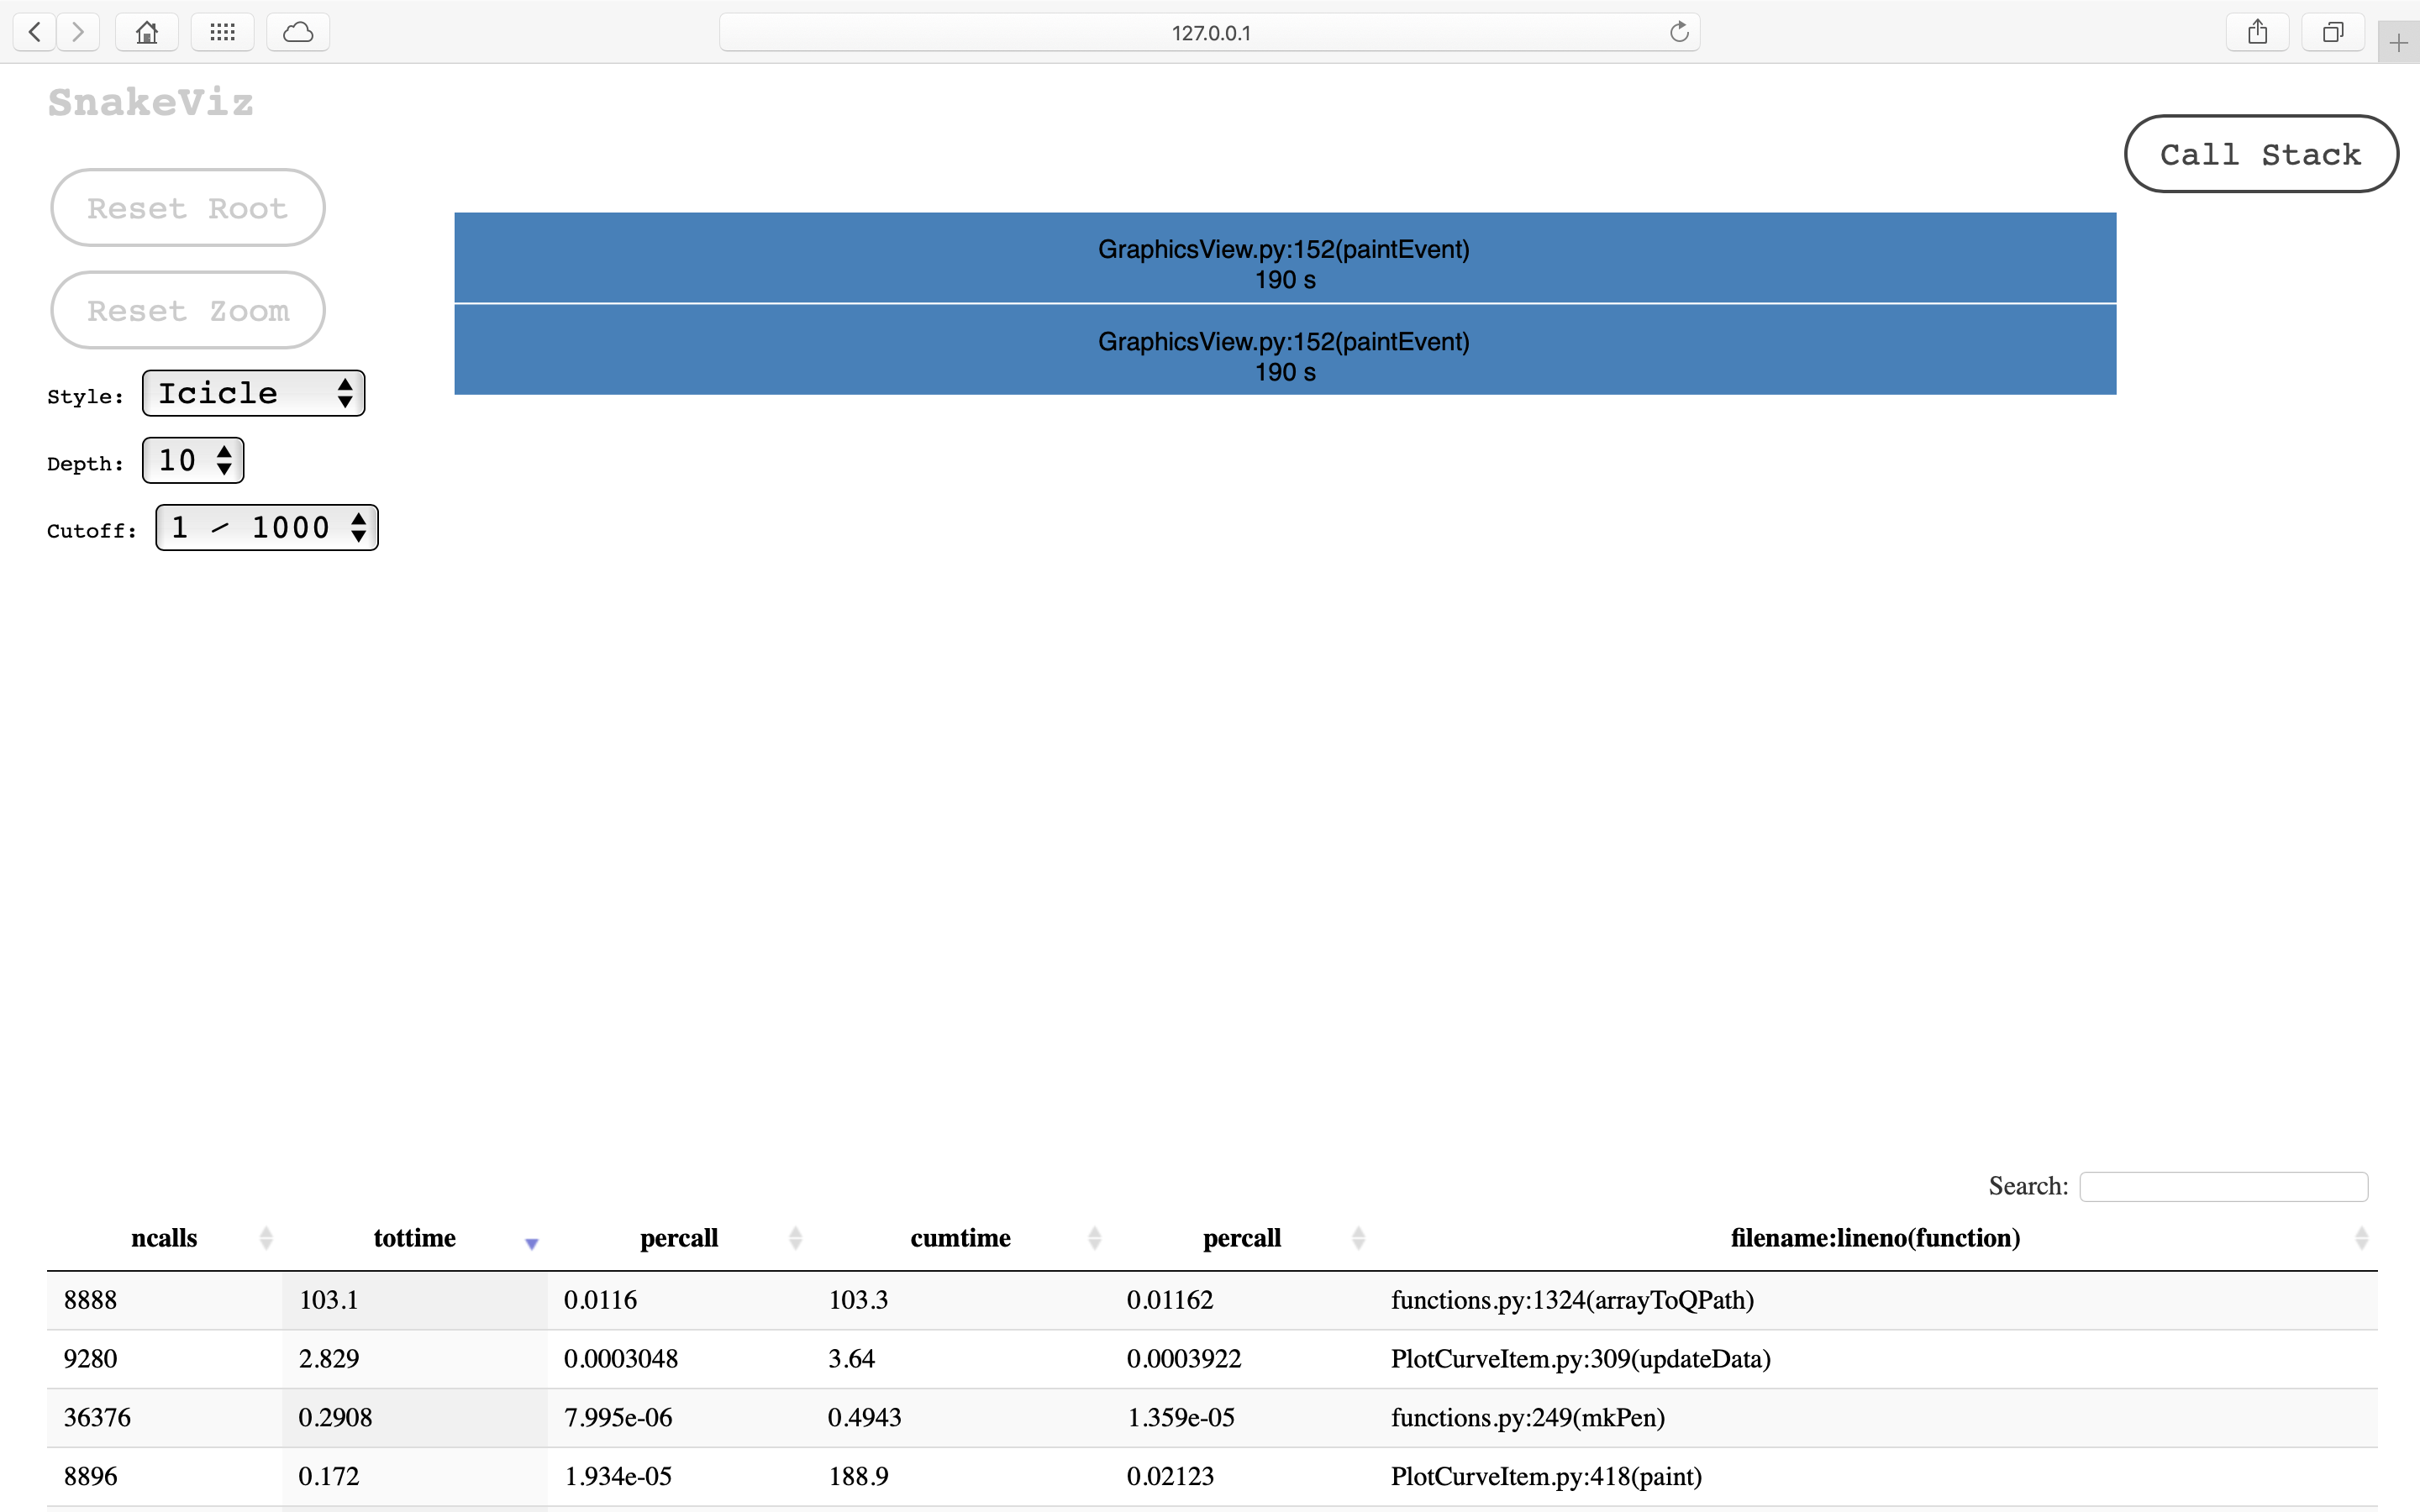
\includegraphics[width=15cm]{resources/img/profiles/HtProfile}
    \caption{Screenshot of the BE-CO-HT use case using Snakeviz}
    \label{fig:application:lhc:usecase:profile:ht}
\end{figure}

When it comes to scatter plots, another function does take quite some time as
well. A big amount of time is spent in the preparation of the symbol atlas,
which is a prerendered image of all symbols used in the scatter plot. When it
comes to rendering the actual plot, the already rendered symbols can simply be
copied from this atlas and pasted into the image. One potential way of improving
performance here is to bypass the loop over each data point in case all symbols
are the same. Screenshot \ref{fig:application:aps:usecase:profile:ht} shows the
profile of the \gls{aps} use case presented by Snakeviz in the browser.

\begin{figure}[h]
    \centering
    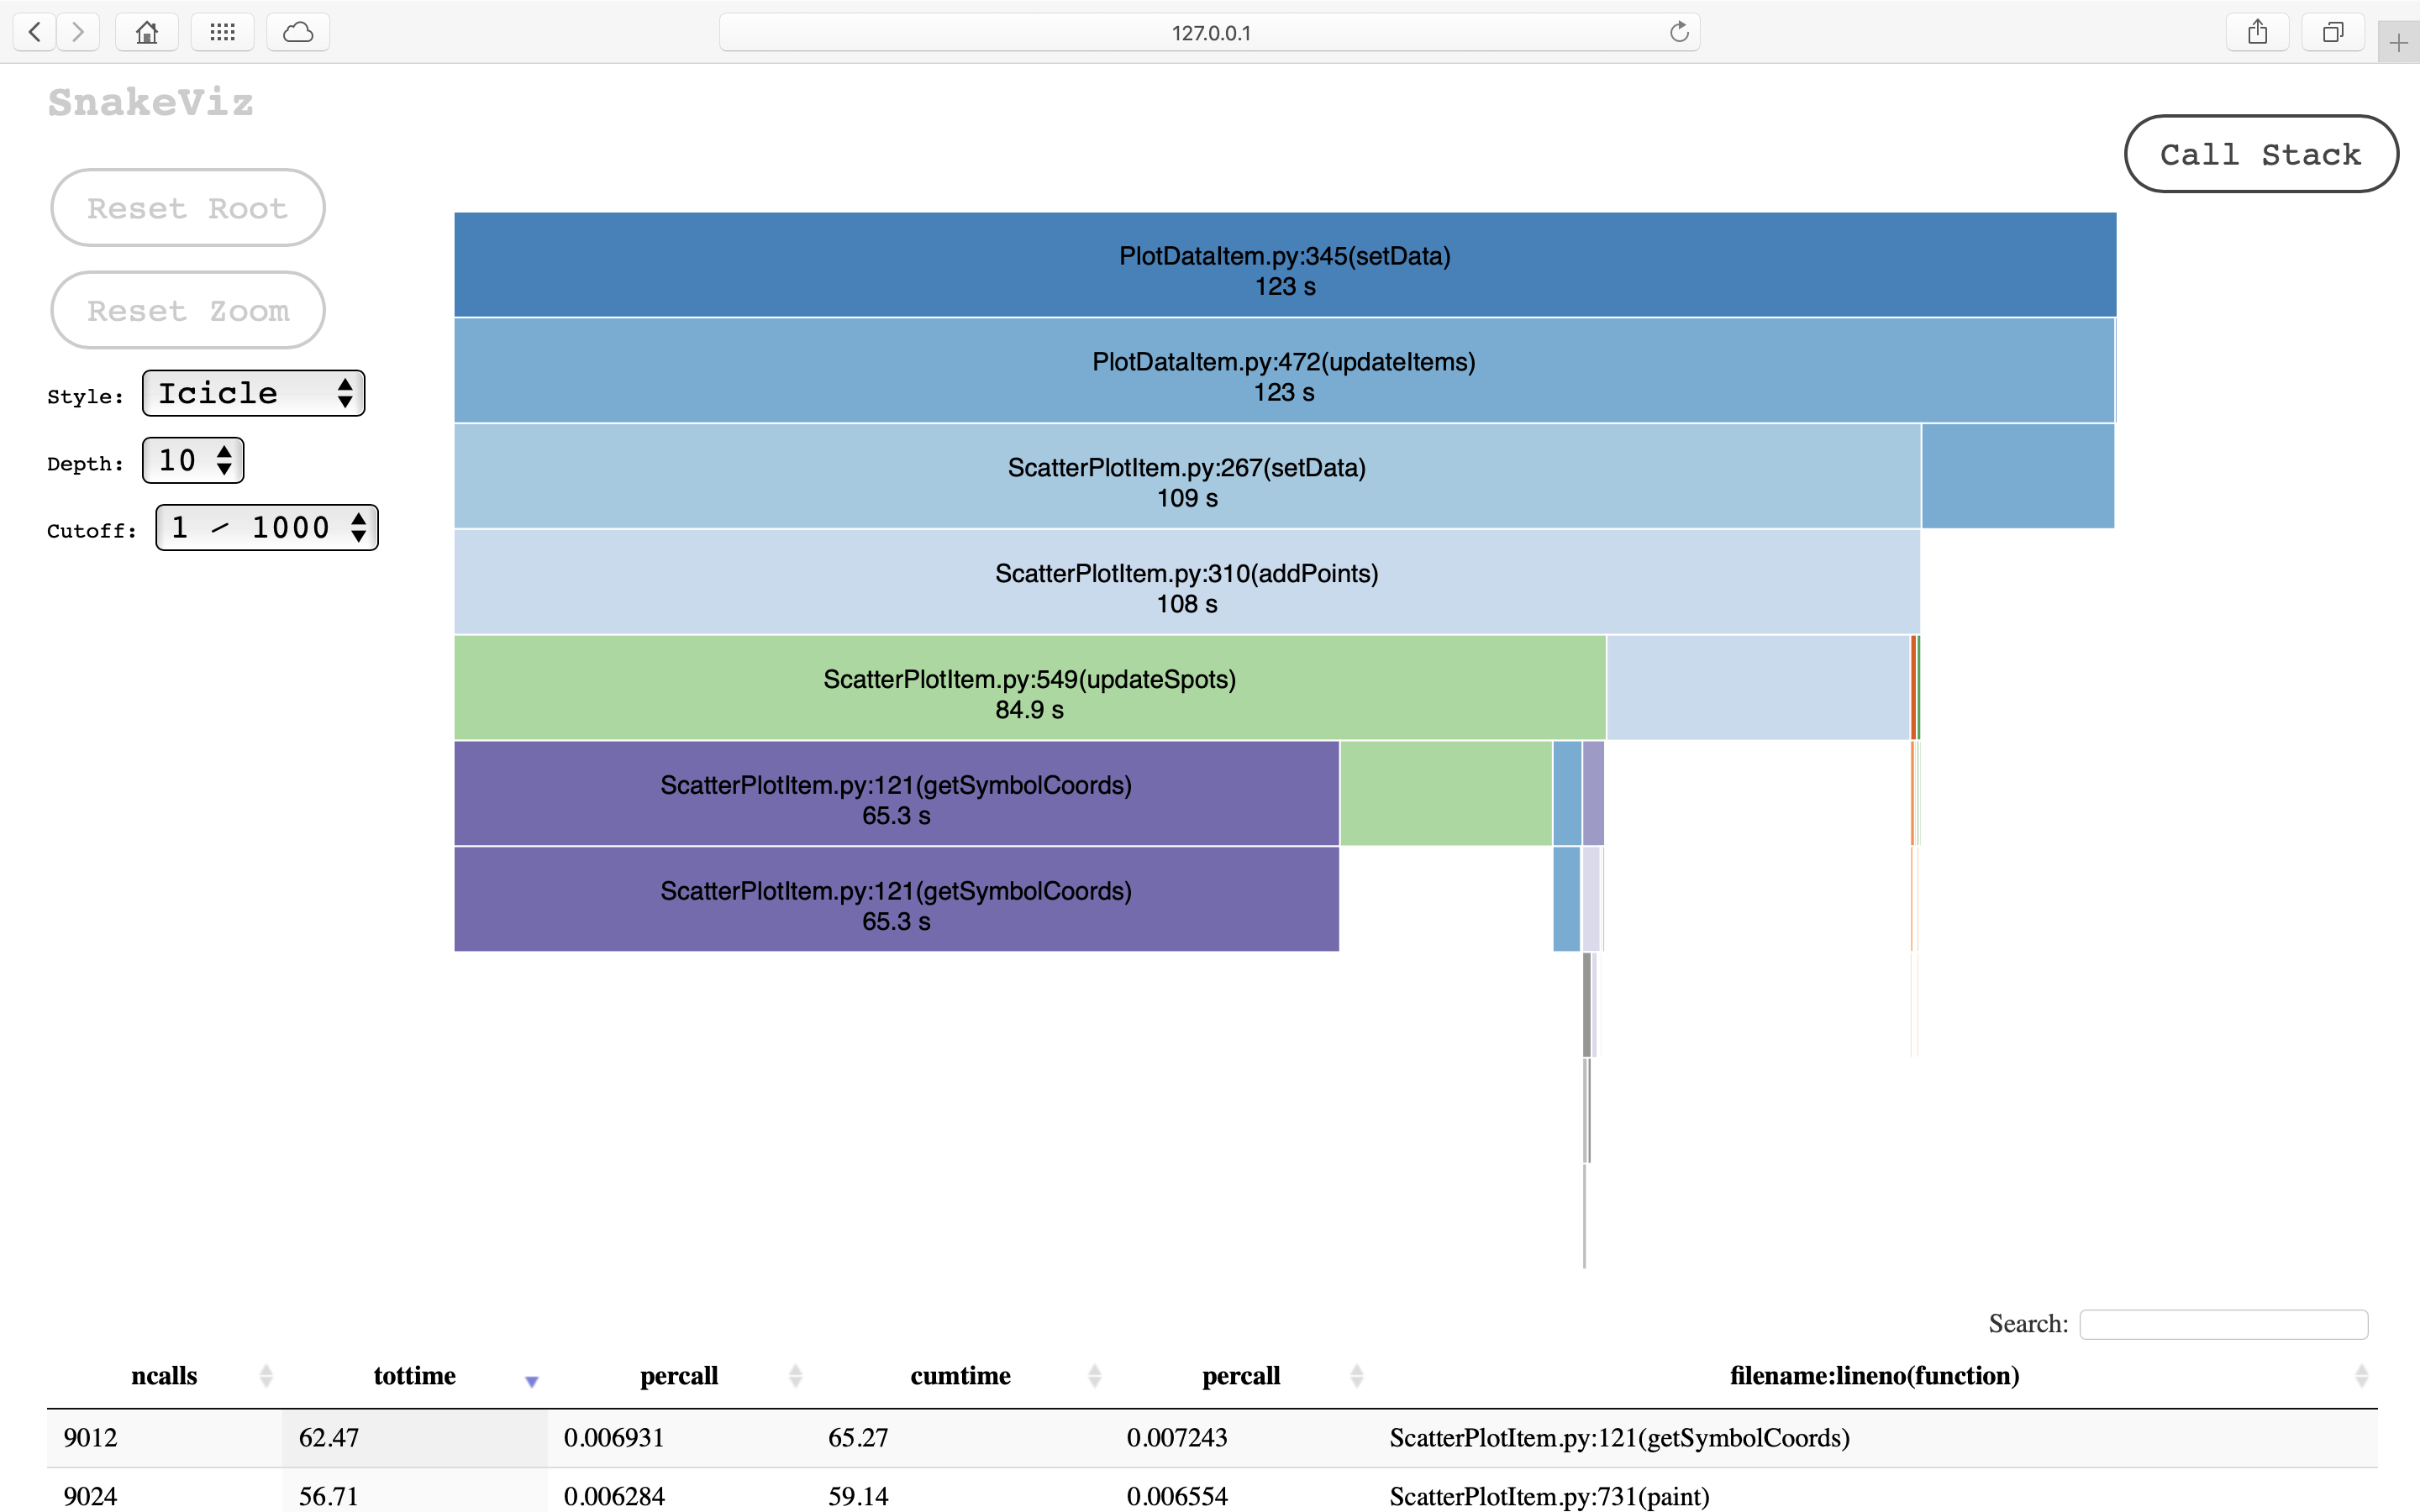
\includegraphics[width=15cm]{resources/img/profiles/ApsProfile}
    \caption{
        Screenshot of the BE-CO-APS use case's profile visualized in snakeviz
    }
    \label{fig:application:aps:usecase:profile:ht}
\end{figure}

\clearpage


%% ==============================================
%%          Performance Overhead
%% ==============================================


\section{Performance Overhead}

This chapter will focus on the evaluation of the framework. The biggest question
when it comes to evaluating performance of widgetmark is, how much overhead it
is adding compared to a standard application. The bigger our overhead is, the
more negative the results will be compared to the realistic value we can expect.

\subsection{Comparison Application}

To evaluate the accuracy of our benchmarking framework, we will compare the
times measured in a simple example use case with an actual implementation as a
minimal PyQt application. This application will only house a single plot updated
by the same conditions as the use case. To measure the timing in the
application, we will record a timestamp after each update. To find out how the
overhead of the framework develops under different load scenarios, we will use
different dataset size parameters for the plotting. For the evaluation we will
only choose a single plotting library, which will be PyQtGraph. The source code
for this application can be seen in listing \ref{listing:evaluation:pyqtapp}. It
is comprised of a single main window, containing the plot as its central widget.
The plot is a \inlinecode{Python}{pyqtgraph.PlotWidget()}, which is updated
using a \inlinecode{Python}{QtCore.QTimer} with a 0 second timeout, similar to
widgetmark's Qt executor class. Next to the data update, the current timestamp
is recorded on every timer timeout. As a hard coded barrier, 1000 redraws are
chosen. For every configuration, we have to executed the python module with
different parameters. The source code for the use case is appended in listing
\ref{listing:evaluation:usecase}. In both cases, the data generation are
excluded from time recording.

\subsection{Delta Time Accuracy}

Table \ref{tab:evaluation} compares the measured frame rates for each use case.
Both variants were executed on the same hardware with the same screen resolution
as well as the same window size. The measured data shows a trend of the
framework being slightly slower compared to the minimal PyQt application.

\begin{table}[h]
\begin{center}

\captionof{table}{
    Frame rate comparison between widgetmark and a minimal PyQt application
}
\label{tab:evaluation}

\begin{tabular}{rrrr}

\hline
Dataset Size & Widgetmark & PyQt Application & Overhead \\
\hline
1000         & 58.8       & 59.8             & 2.2\%    \\
10000        & 59.7       & 59.6             & 0\%      \\
500000       & 23.8       & 25.9             & 8.1\%    \\
1000000      & 12.5       & 13.9             & 10.1\%   \\
\hline

\end{tabular}
\end{center}
\end{table}

While these measurements already provide us with a general trend of the
framework adding a small overhead to our execution, it raises the question, how
this deviation compares with the fluctuation of the recorded times within a
execution. To compare this we first will have to get access to all measured
delta times for the PyQt application as well as the widgetmark run.

As a small rehearsal, we will quickly explain the sizes used in the following
detailed evaluation and why they are meaningful for us. The first important
measurement is the delta timing $\Delta t$, which describes the difference
between two measured adjacent time stamps. From a set of $m$ timestamps it can
be calculated for two adjacent timestamps $t_{i+1}$ and $t_i$ as:

$$\Delta t_{i} = t_{i+1} - t_{i}$$

The arithmetic mean or average $\bar{\Delta t}$ describes the average from our
set of $m-1$ measured delta times and is defined as:

$$\bar{\Delta t} = \frac{1}{m-1} * \sum_{i=0}^{m-1} {\Delta t_{i}}$$

The standard deviation $\sigma$ of our delta times describes, how far values are
deviated on average from $\bar{\Delta t}$. From the standard $\sigma$ we can get
a better idea if the measured times are very consistent or if they differ much
from each other. It is defined as:

$$ \sigma_{\Delta t} = \sqrt{\frac{1}{m-2} * \sum_{i=1}^{m-2} (\Delta t_{i} - \bar{\Delta t})^2} $$

The range of a set of $m-1$ delta times $\Delta t_i$ describes the difference
between the largest and smallest measured $\Delta t$ and is defined as:

$$R_{\Delta t} = \Delta t_{max} - \Delta t_{min}$$

Figures \ref{a:tab:evaluation:1000}, \ref{a:tab:evaluation:10000},
\ref{a:tab:evaluation:50000} and \ref{a:tab:evaluation:100000} compare all
measured delta times in the widgetmark as well as the minimal PyQt application.
For smaller dataset sizes, there are only small difference between both
noticeable. If the dataset size however increases, the difference measured in
the frame rates can be seen very well. In figure \ref{fig:evaluation:avg}, which
shows the average of the measured delta times, this difference becomes more
apparent.

\begin{figure}[h]
    \centering
    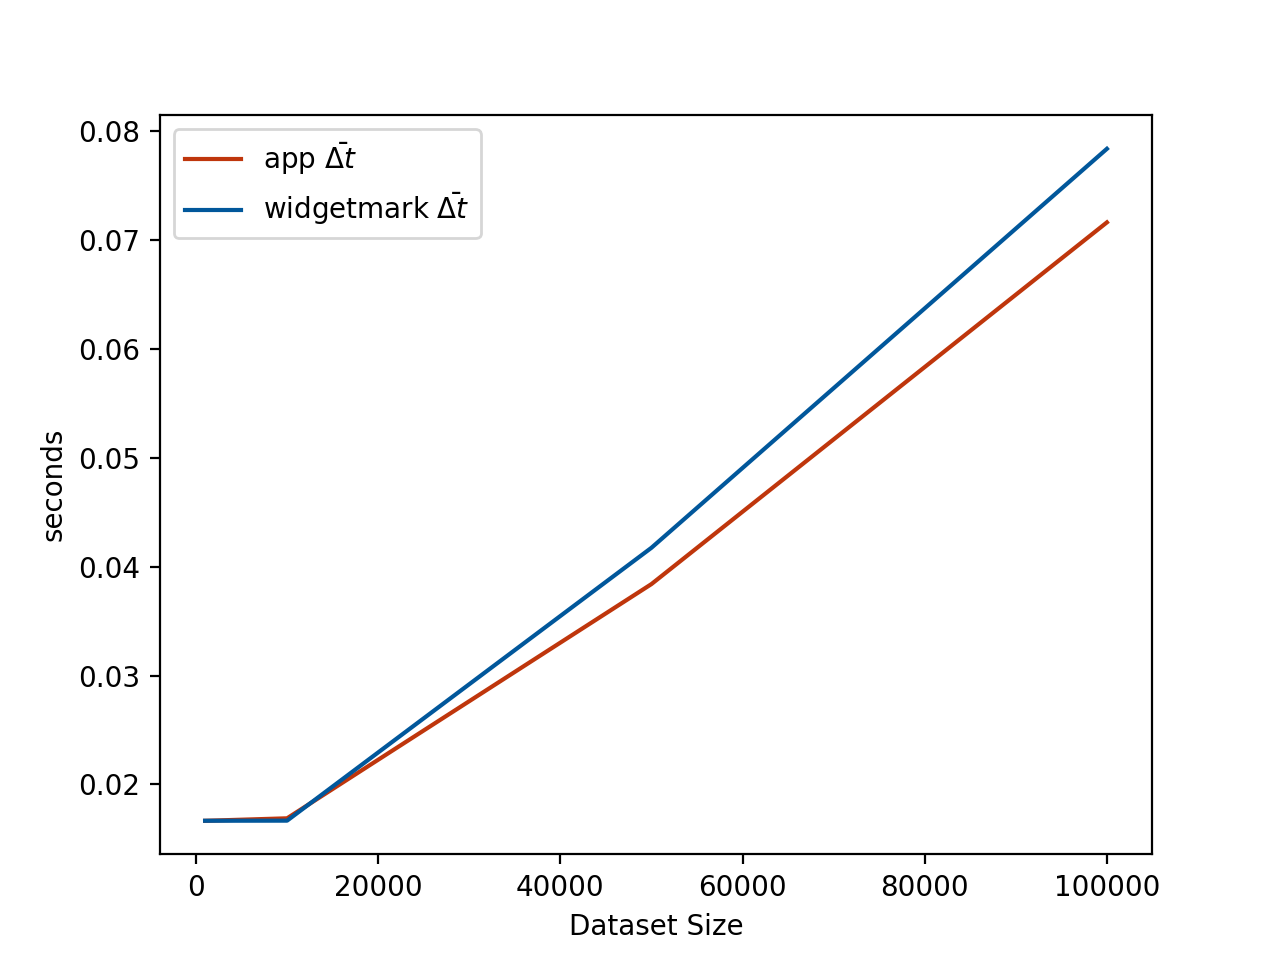
\includegraphics[width=12cm]{resources/img/evaluation/Eval_AVG}
    \caption{Average delta timing between both execution variants}
    \label{fig:evaluation:avg}
\end{figure}

Figure \ref{fig:evaluation:std} compares the difference between the average
delta times, the fluctuation of measured individual delta times and the ranges
$R_{\Delta t}$ of the framework as well as the minimal application. The
difference between widgetmark and the app in $\bar{\Delta t}$ is bigger compared
to their individual standard deviations $\sigma_{\Delta t}$. If it was in this
deviation range, it would be much more likely to be just a fluctuation in our
measurements. By clearly exceeding the expected deviation, we can assume that
the overhead will be reproducible, which supports our assumption, that
widgetmark does add an additional overhead to the execution, especially for
larger data set sizes. Compared to the measured value ranges $R_{\Delta t}$ of
each run, the difference is considerably smaller. These large ranges clearly
show, that it is very hard to further estimate, how high this actual overhead
will be on a run, since the recorded delta times can be very heavily influenced
by factors like the current load on the system. This is especially well
represented by the exceptional high range for the comparison application at
a data set size of $50000$ points. Additionally it shows the importance of a
reasonably high repeat counter, to keep the influence of such stray bullets as
small as possible.

\begin{figure}[h]
    \centering
    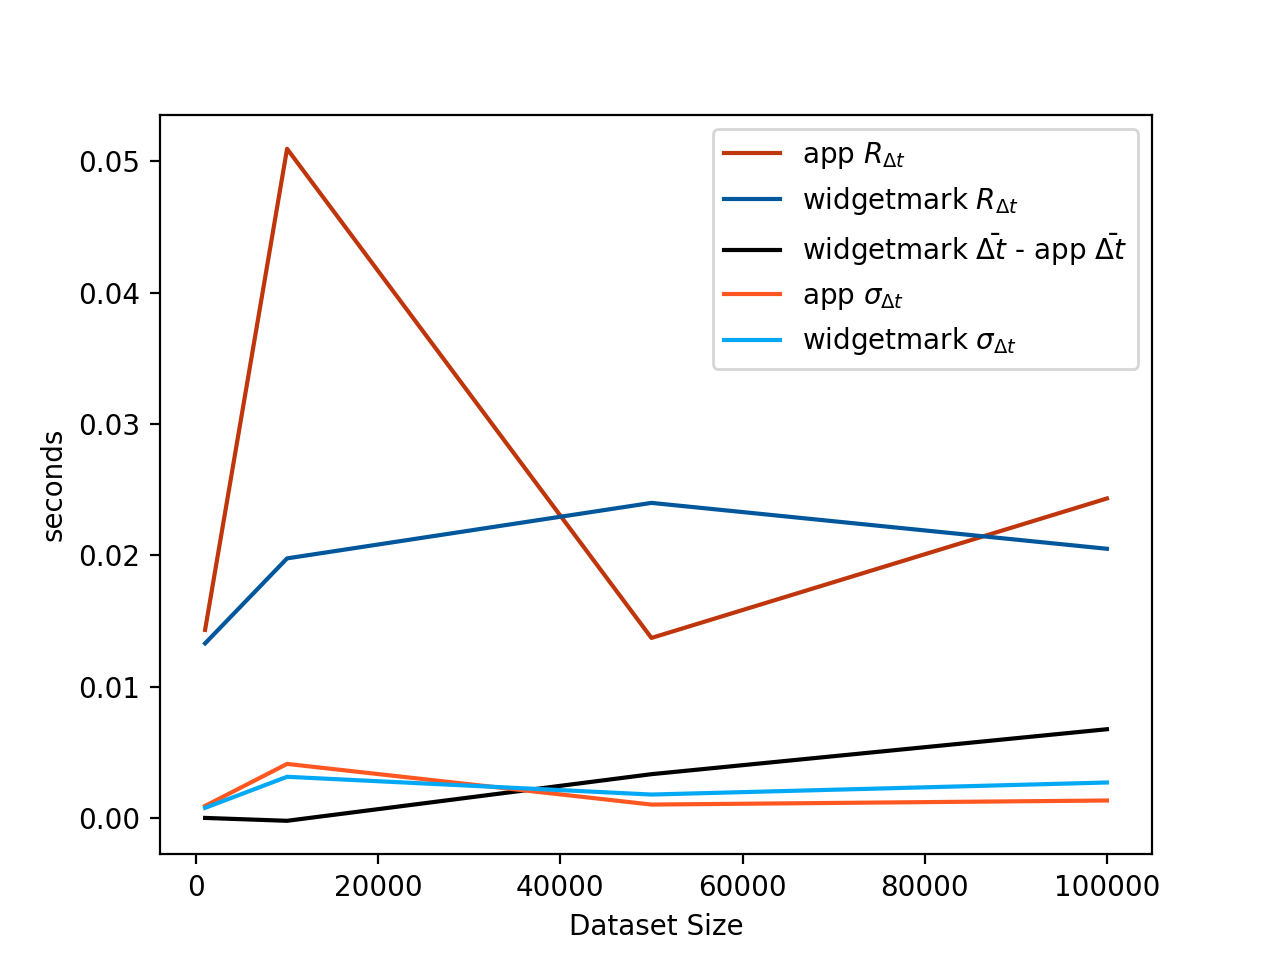
\includegraphics[width=12cm]{resources/img/evaluation/Eval_STD}
    \caption{Standard deviation compared to the delta timing value ranges and
        the average delta timing difference between both execution variants}
    \label{fig:evaluation:std}
\end{figure}

As a summary for the evaluation we can see, that widgetmark does add a slight
overhead to the executed use case. This overhead however does only slightly
influence the outcome of each use case, since it is still manages to represent
the libraries realistic performance capabilities.

%% LaTeX2e class for student theses
%% sections/conclusion.tex
%%
%% Karlsruhe University of Applied Sciences
%% Faculty of  Computer Science and Business Information Systems
%% Distributed Systems (vsys)
%%
%% Prof. Dr. Christian Zirpins
%% christian.zirpins@hs-karlsruhe.de
%%
%%
%% Version 0.2, 2017-11-15
%%
%% --------------------------------------------------------
%% | Derived from sdqthesis by Erik Burger burger@kit.edu |
%% --------------------------------------------------------


\chapter{Conclusion}
\label{ch:Conclusion}

\section{Summary}
\label{sec:Conclusion:Summary}

\dots

\section{Outlook}
\label{sec:Conclusion:Outlook}

\dots



%% --------------------
%% |   Bibliography   |
%% --------------------

%% Add entry to the table of contents for the bibliography
\printbibliography[heading=bibintoc]


%% ----------------
%% |   Appendix   |
%% ----------------
\appendix
\iflanguage{english}
{\chapter{Appendix}}    % english style
{\chapter{Anhang}}      % german style
\label{chap:appendix}

\section{PyQt}
\label{sec:appendix:pyqt}

\setcounter{figure}{0}

\lstinputlisting[
    language=python,
    caption=Source code for the layout example in \ref{fig:qt:examplewindow}, 
    label=a:fig:qt:examplewindow:code
]{resources/code/windowexample.py}

\lstinputlisting[
    language=python,
    caption=Source code an example window demonstrating qts event system,
    label=a:qtevents:code
]{resources/code/event_complete.py}

\clearpage

\section{PyQtGraph}
\label{sec:appendix:pyqtgraph}

\begin{figure}[h]
    \centering
    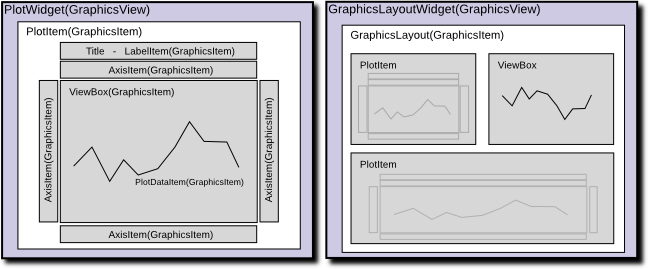
\includegraphics[width=14cm]{resources/img/PyQtGraphContent}
    \caption{Different items involved in a PlotWidget.}
    \small\textsuperscript{Quelle: http://www.pyqtgraph.org/documentation/plotting.html}
    \label{a:fig:pyqtgraph:content}
\end{figure}

\begin{figure}[h]
    \centering
    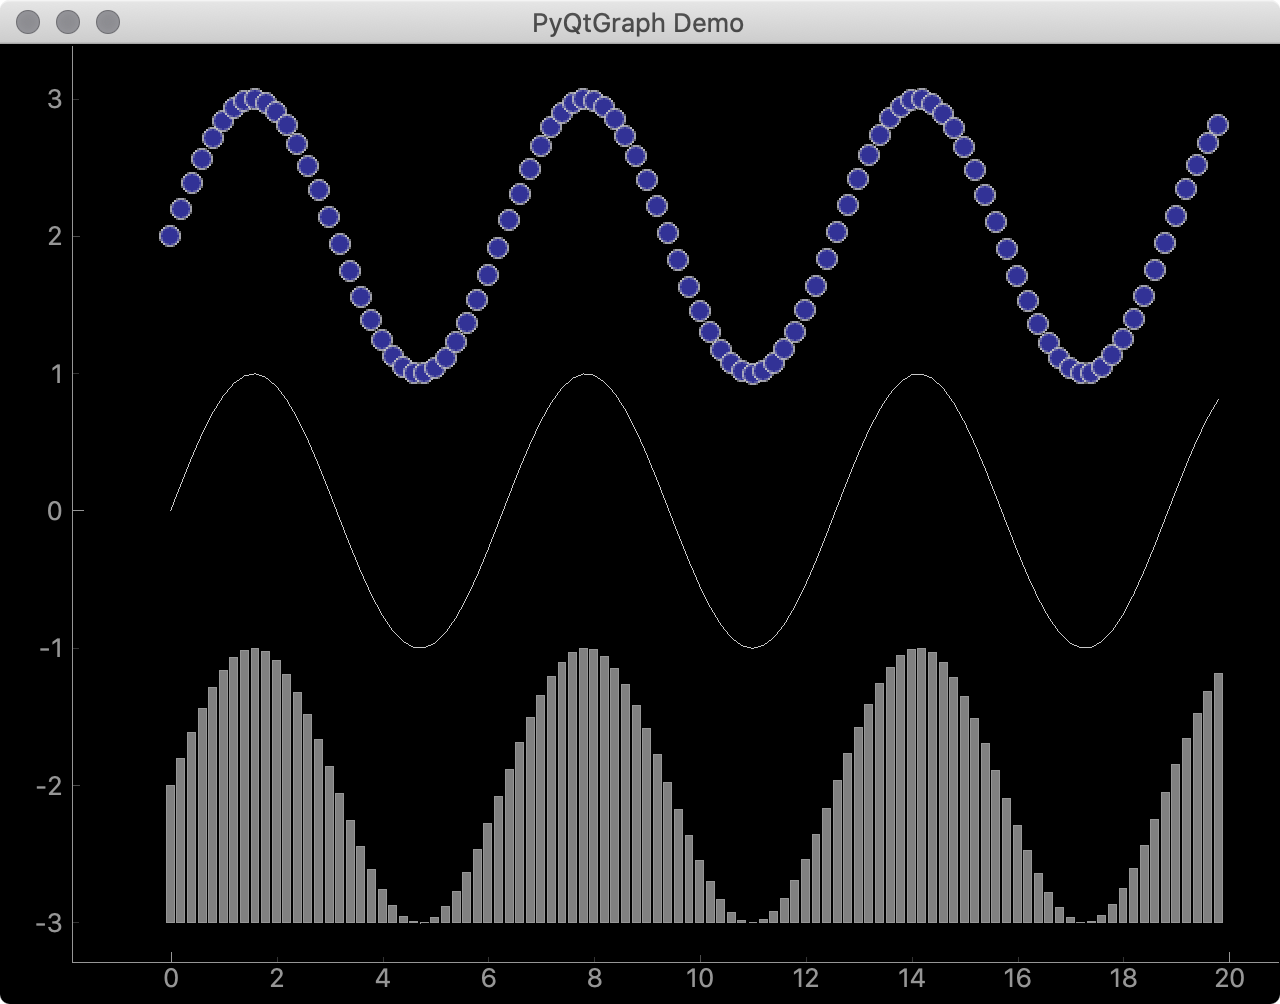
\includegraphics[width=14cm]{resources/img/PyQtGraphDemo}
    \caption{Window containing a plot created with PyQtGraph.}
    \label{a:fig:pyqtgraph:window}
\end{figure}

\clearpage

\section{Matplotlib}
\label{sec:appendix:matplotlib}

\begin{figure}[h]
    \centering
    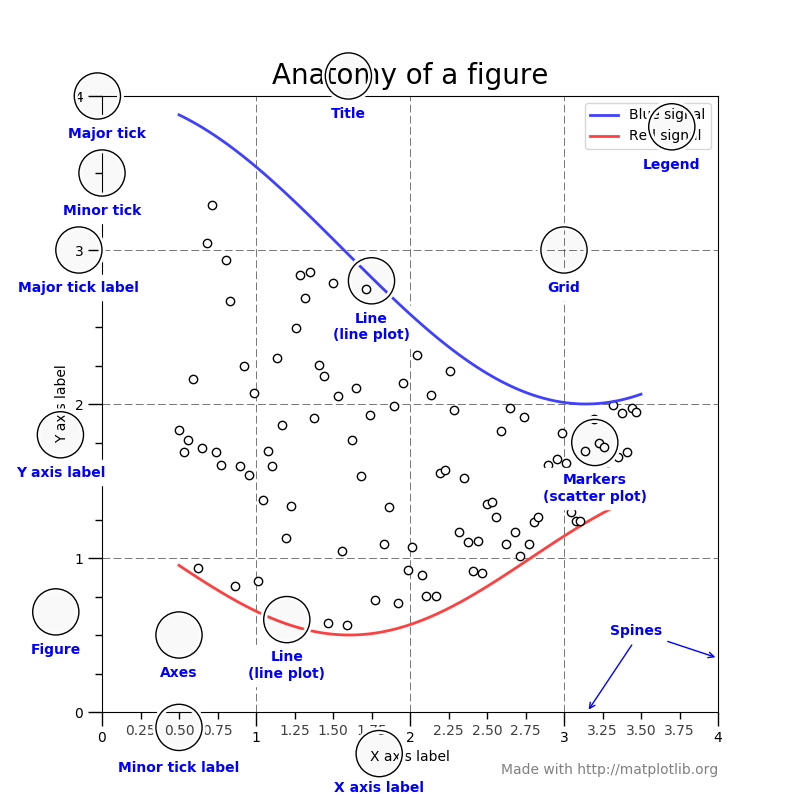
\includegraphics[width=14cm]{resources/img/MatplotlibContent}
    \caption{Different items involved in a Figure.}
    \small\textsuperscript{Quelle: https://matplotlib.org/3.1.1/tutorials/introductory/usage.html}
    \label{a:fig:matplotlib:content}
\end{figure}

\begin{figure}[h]
    \centering
    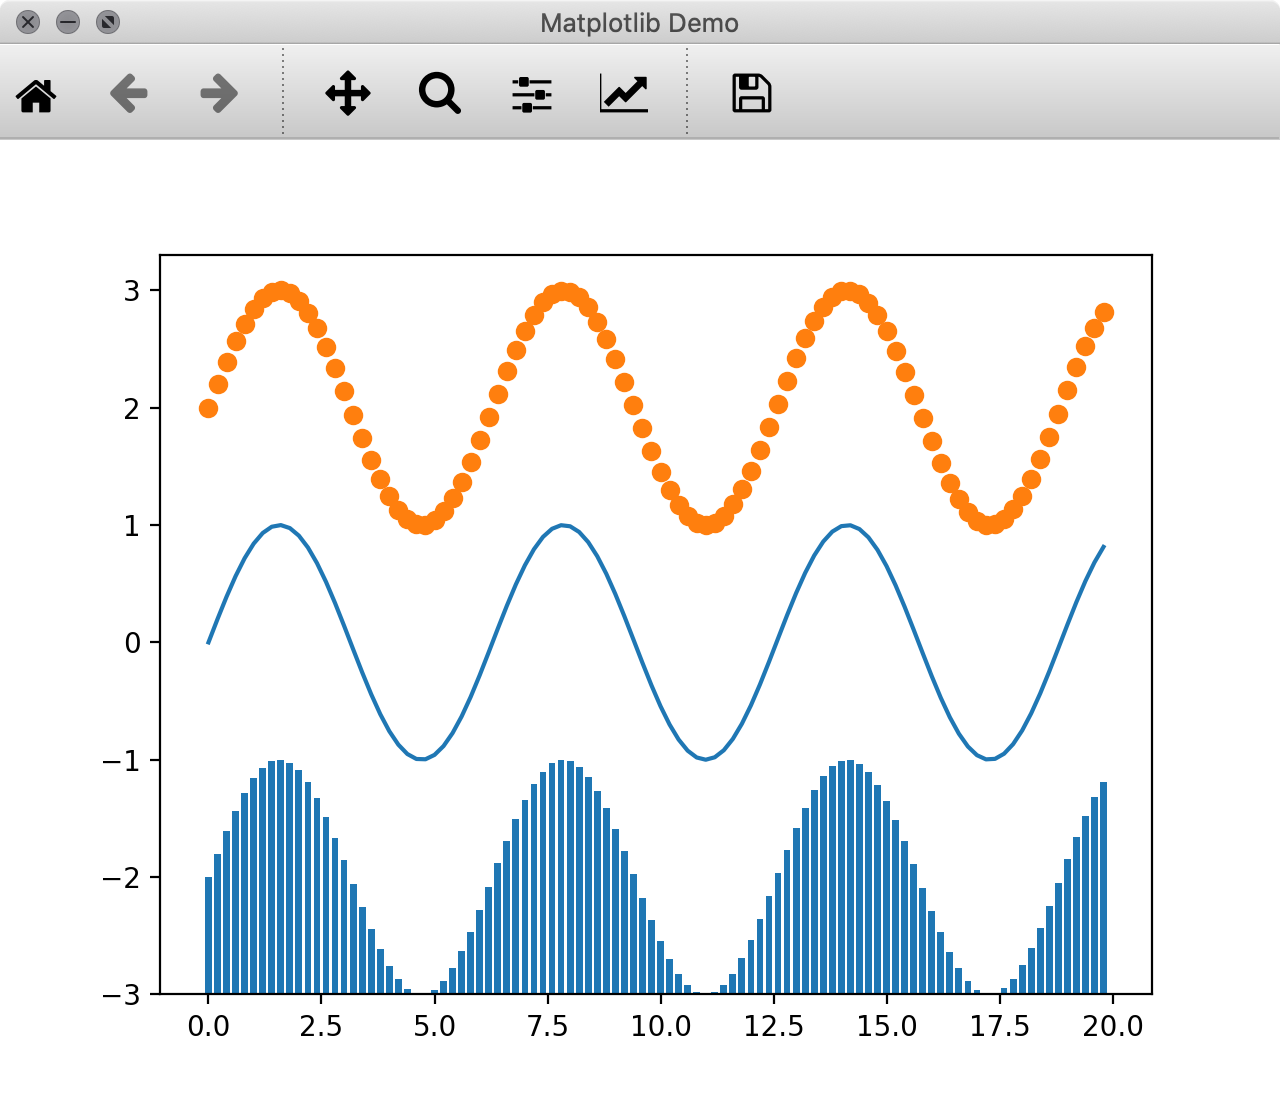
\includegraphics[width=14cm]{resources/img/MatplotlibDemo}
    \caption{Window containing plot created with Matplotlib.}
    \label{a:fig:matplotlib:window}
\end{figure}

\clearpage

\section{Evaluation}
\label{sec:appendix:evaluation}

\begin{figure}[h]
    \centering
    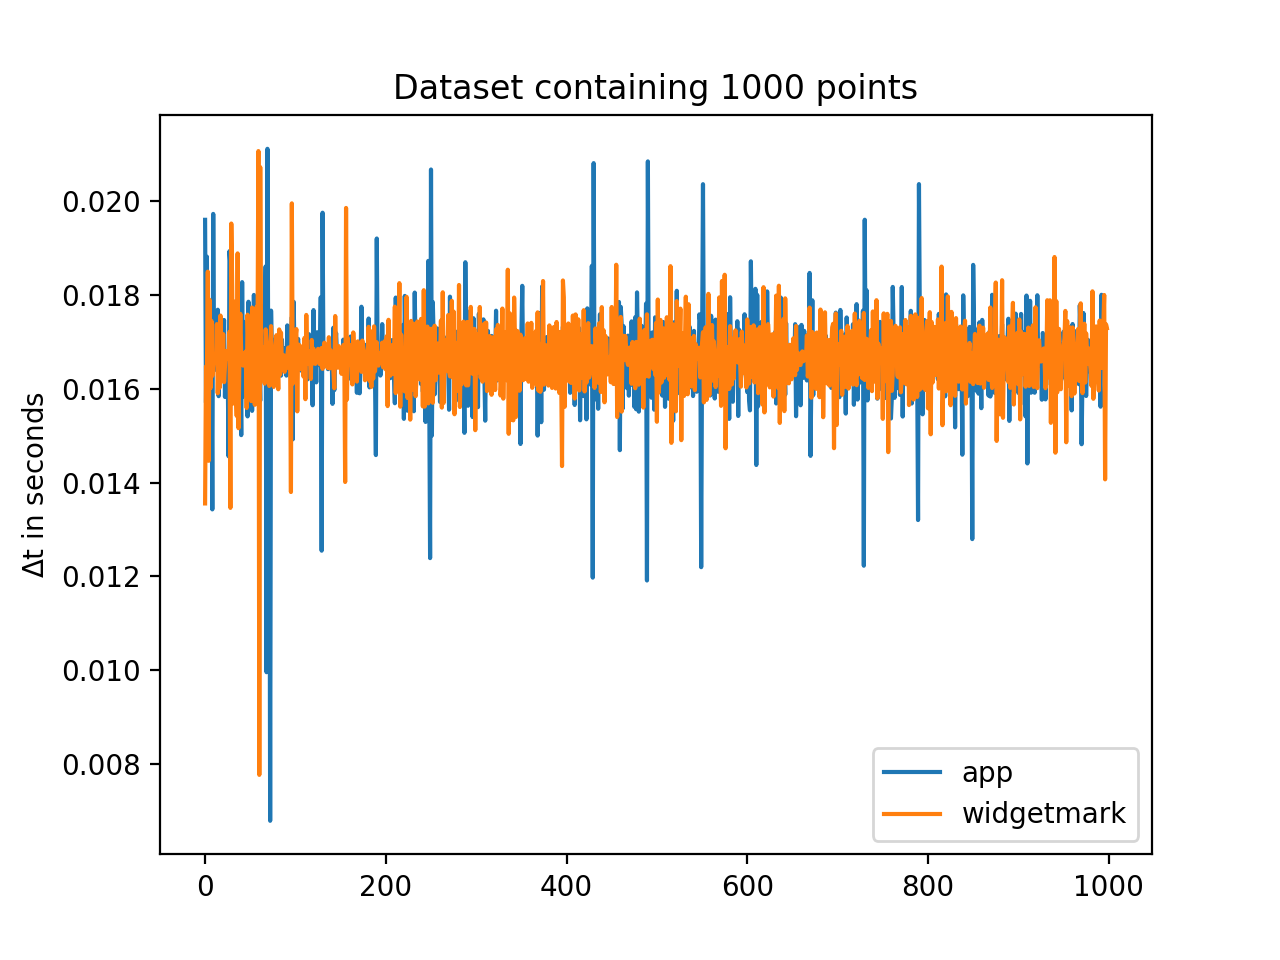
\includegraphics[width=12cm]{resources/img/evaluation/Eval_1000}
    \caption{
        Recorded Delta Times of for 1000 points
    }
    \label{a:tab:evaluation:1000}
\end{figure}


\begin{figure}[h]
    \centering
    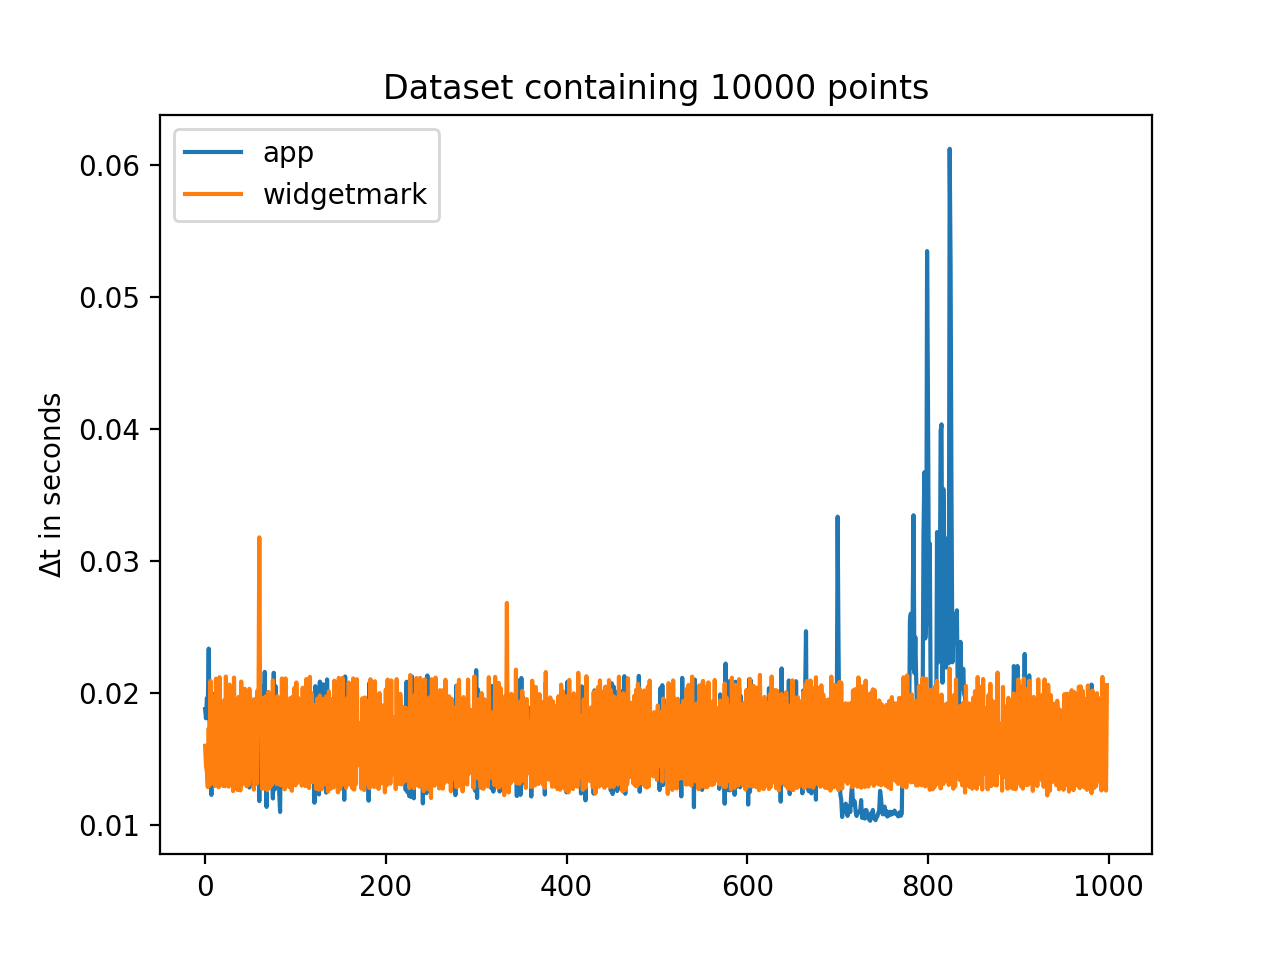
\includegraphics[width=12cm]{resources/img/evaluation/Eval_10000}
    \caption{
        Recorded Delta Times of for 10,000 points
    }
    \label{a:tab:evaluation:10000}
\end{figure}


\begin{figure}[h]
    \centering
    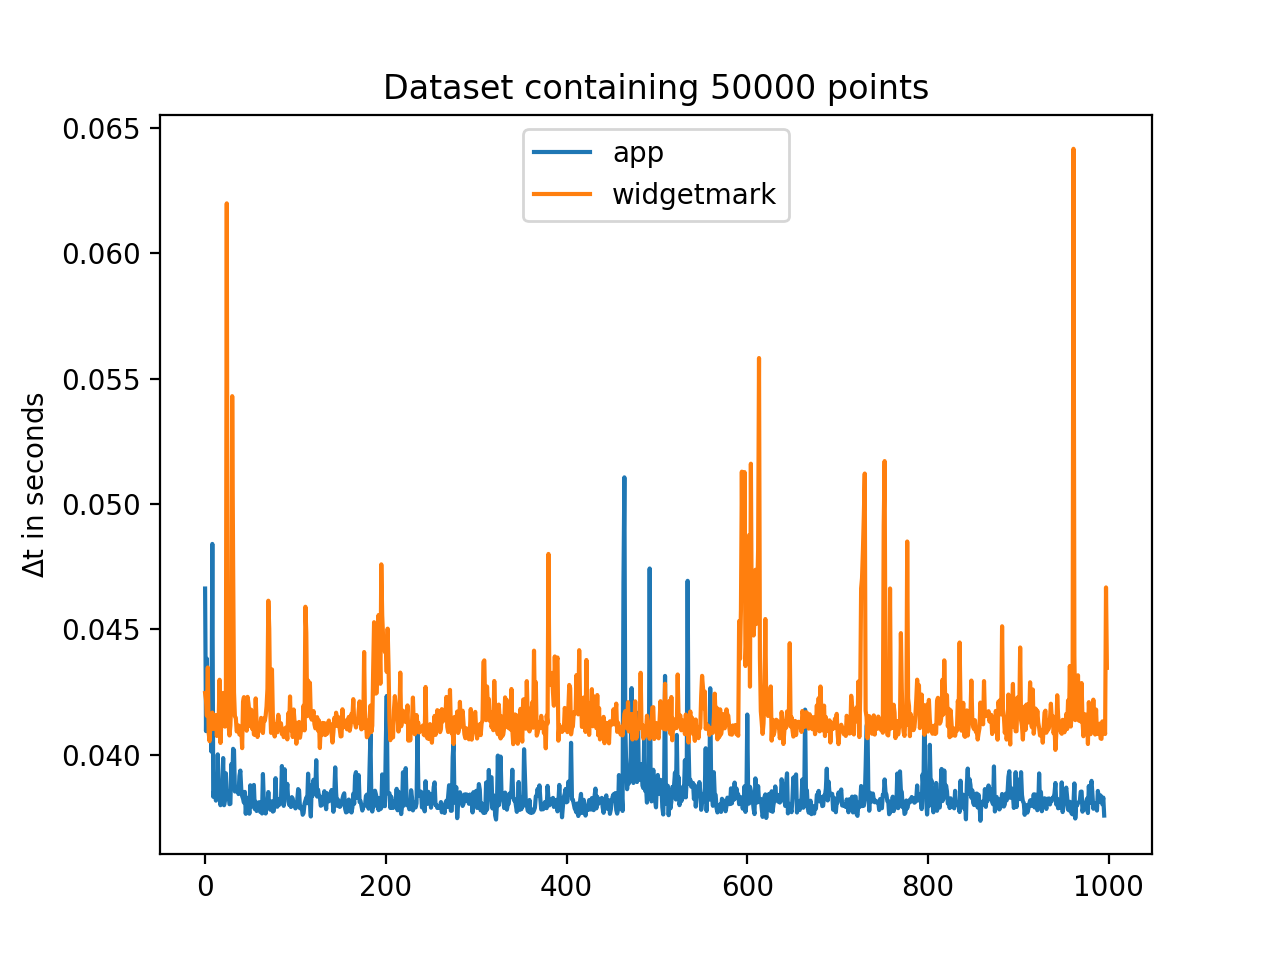
\includegraphics[width=12cm]{resources/img/evaluation/Eval_50000}
    \caption{
        Recorded Delta Times of for 50,000 points
    }
    \label{a:tab:evaluation:50000}
\end{figure}


\begin{figure}[h]
    \centering
    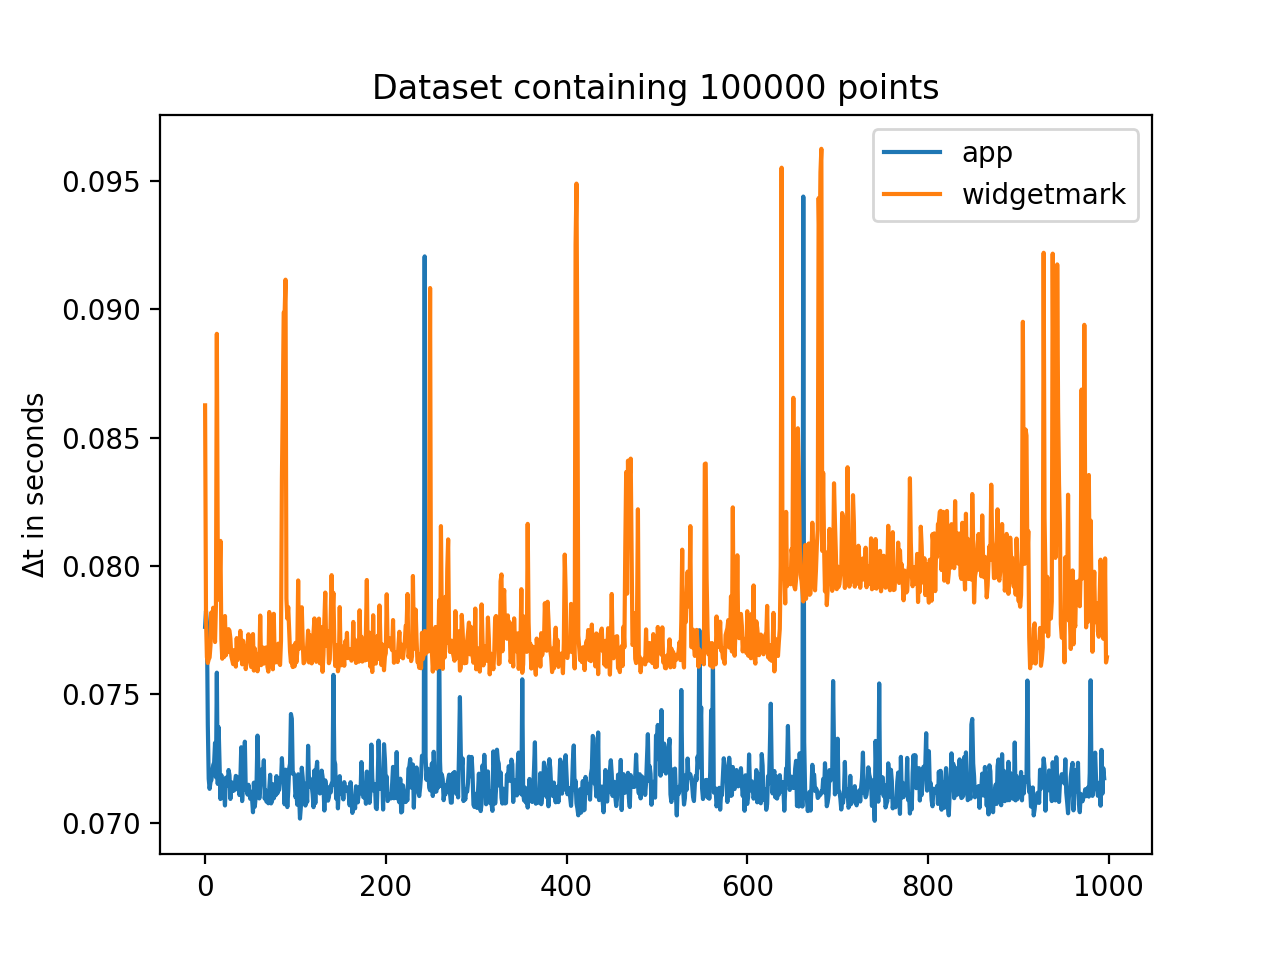
\includegraphics[width=12cm]{resources/img/evaluation/Eval_100000}
    \caption{
        Recorded Delta Times of for 100,000 points
    }
    \label{a:tab:evaluation:100000}
\end{figure}


%% Evaluation Code
\clearpage

\lstinputlisting[
    caption=PyQt comparison application,
    language=python, 
    label=listing:evaluation:pyqtapp
]{resources/widgetmark/evaluation/app.py}


\lstinputlisting[
    caption=Evaluation use case for widgetmark,
    language=python, 
    label=listing:evaluation:usecase
]{resources/widgetmark/evaluation/usecase.py}

%% ---------------------
%% | / Example content |
%% ---------------------


\end{document}
